%%
%% Copyright 2007-2025 Elsevier Ltd
%%
%% This file is part of the 'Elsarticle Bundle'.
%% ---------------------------------------------
%%
%% It may be distributed under the conditions of the LaTeX Project Public
%% License, either version 1.3 of this license or (at your option) any
%% later version.  The latest version of this license is in
%%    http://www.latex-project.org/lppl.txt
%% and version 1.3 or later is part of all distributions of LaTeX
%% version 1999/12/01 or later.
%%
%% The list of all files belonging to the 'Elsarticle Bundle' is
%% given in the file `manifest.txt'.
%%
%% Template article for Elsevier's document class `elsarticle'
%% with numbered style bibliographic references
%% SP 2008/03/01
%% $Id: elsarticle-template-num.tex 272 2025-01-09 17:36:26Z rishi $
%%
\documentclass[preprint,12pt]{elsarticle}

%% Use the option review to obtain double line spacing
%% \documentclass[authoryear,preprint,review,12pt]{elsarticle}

%% Use the options 1p,twocolumn; 3p; 3p,twocolumn; 5p; or 5p,twocolumn
%% for a journal layout:
%% \documentclass[final,1p,times]{elsarticle}
%% \documentclass[final,1p,times,twocolumn]{elsarticle}
%% \documentclass[final,3p,times]{elsarticle}
%% \documentclass[final,3p,times,twocolumn]{elsarticle}
%% \documentclass[final,5p,times]{elsarticle}
%% \documentclass[final,5p,times,twocolumn]{elsarticle}

%% For including figures, graphicx.sty has been loaded in
%% elsarticle.cls. If you prefer to use the old commands
%% please give \usepackage{epsfig}
\usepackage{amssymb}
\usepackage{amsmath}
\usepackage{amsthm}
\usepackage{algorithm}
\usepackage{algorithmic}
\usepackage{booktabs}
\usepackage{float}
\usepackage{graphicx}
\usepackage{pdfpages}
\usepackage{multirow}
\usepackage{url}
%\journal{Journal of Computational Physics}
\usepackage[colorlinks=true,        % 使用彩色文字代替边框
            linkcolor=blue,         % 内部链接颜色
            citecolor=red,          % 引用颜色
            urlcolor=magenta,       % URL 颜色
            filecolor=cyan,         % 文件链接颜色
            bookmarks=true,         % 生成书签
            bookmarksopen=true,     % 展开书签
            bookmarksnumbered=true, % 书签带编号
            pdftitle={Discovery-Informed NoProp: Transferring Discovered Physical Relations into Local Learning},
            pdfauthor={Jianfeng Wu and Jun Guo}]{hyperref}

\begin{document}
\setlength{\emergencystretch}{3em}

\begin{frontmatter}

%% Title, authors and addresses

%% use the tnoteref command within \title for footnotes;
%% use the tnotetext command for theassociated footnote;
%% use the fnref command within \author or \affiliation for footnotes;
%% use the fntext command for theassociated footnote;
%% use the corref command within \author for corresponding author footnotes;
%% use the cortext command for theassociated footnote;
%% use the ead command for the email address,
%% and the form \ead[url] for the home page:
%% \title{Title\tnoteref{label1}}
%% \tnotetext[label1]{}
%% \author{Name\corref{cor1}\fnref{label2}}
%% \ead{email address}
%% \ead[url]{home page}
%% \fntext[label2]{}
%% \cortext[cor1]{}
%% \affiliation{organization={},
%%             addressline={},
%%             city={},
%%             postcode={},
%%             state={},
%%             country={}}
%% \fntext[label3]{}

\title{Discovery-Informed NoProp: Transferring Discovered Physical Relations into Local Learning}

% use optional labels to link authors explicitly to addresses:
% \author[label1,label2]{}
% \affiliation[label1]{organization={},
%             addressline={},
%             city={},
%             postcode={},
%             state={},
%             country={}}
%
% \affiliation[label2]{organization={},
%             addressline={},
%             city={},
%             postcode={},
%             state={},
%             country={}}

 %% Author name
\author[inst1]{Jianfeng Wu}
\author[inst2,inst3]{Jun Guo\corref{cor1}}
\cortext[cor1]{Corresponding author}
%% Author affiliation

\affiliation[inst1]{organization={Chengdu University of Information Technology},
            city={Chengdu},
            postcode={610225},
            % state={Sichuan},
            country={China}}
            
\affiliation[inst2]{organization={College of Applied Mathematics, Chengdu University of Information Technology},
            city={Chengdu},
            postcode={610225},
            % state={Sichuan},
            country={China}}

\affiliation[inst3]{organization={Key Laboratory of Mathematical Meteorology, Chengdu University of Information Technology},
            city={Chengdu},
            postcode={610225},
            % state={Sichuan},
            country={China}}
% \affiliation[inst1]{organization={School of Software Engineering, Chengdu University of Information Technology},
%             % addressline={No. 24, Section 1, Xuefu Road, Southwest Airport Economic Development Zone},
%             city={Chengdu},
%             postcode={610225},
%             % state={Sichuan},
%             country={China}}
% \affiliation[inst2]{organization={School of Sciences, Southwest Petroleum University},
% city={Chengdu},
% postcode={610500},
% state={Sichuan},
% country={China}}

% \affiliation[inst2]{organization={School of Statistics, Chengdu University of Information Technology},
%             % addressline={No. 24, Section 1, Xuefu Road, Southwest Airport Economic Development Zone},
%             city={Chengdu},
%             postcode={610103},
%             % state={Sichuan},
%             country={China}}




\begin{abstract}
Neural network training via back-propagation requires global gradient propagation across all layers, imposing memory overhead and sequential dependencies. We present a discovery-informed NoProp framework in which independently optimised denoising blocks receive local weak-form physical constraints. A dimensionally constrained SPIDER library is evaluated on 60 archived homogeneous-isotropic-turbulence (HIT) snapshots and selected by sparse null-space regression; the resulting relation is tested on 20 disjoint snapshots and under 100 bootstrap resamples. SPIDER selects the pressure-Laplacian and convection-divergence terms with normalized coefficients $(1,0.293)$, validation residual $0.286$, and 100\% support stability. This validated artifact is loaded directly by the trainer and converted into a differentiable local residual; invalid artifacts are rejected without analytic fallback. The implementation samples one block per mini-batch, giving an unbiased estimator of the summed local objective while eliminating cross-block gradients. Three-seed experiments compare vanilla local NoProp, an analytically prescribed pressure--Poisson prior, and the SPIDER-discovered relation. The discovered constraint improves physical consistency but does not improve mean classification accuracy on the present internal overlapping-crop split. The contribution is therefore a verified discovery-to-local-learning pipeline rather than a claim of full Navier--Stokes recovery or independent-trajectory generalisation.
\end{abstract}


%% Keywords
\begin{keyword}
%% keywords here, in the form: keyword \sep keyword
Physics-informed learning\sep  Weak formulation\sep  Sparse regression\sep Turbulent flow \sep  Diffusion models
\end{keyword}

\end{frontmatter}

%% main text
%%
% \clearpage % 强制换页，并输出所有未排版的图表
%% Use \section commands to start a section

\section{Introduction}

Deep neural networks have achieved remarkable successes across a wide range of scientific and industrial domains, largely driven by the effectiveness of back-propagation (BP) for training multi-layer architectures \cite{rumelhart1986learning}. BP iteratively adjusts network parameters by propagating an error signal from the output back through all layers, enabling end-to-end optimization of complex models. Despite its empirical success, BP suffers from several fundamental limitations. First, it is biologically implausible, as it requires symmetric forward and backward passes that do not align with local synaptic plasticity observed in the brain \cite{grossberg1987competitive,lillicrap2016random}. Second, BP necessitates storing intermediate activations during the forward pass, imposing significant memory overhead that hampers scalability \cite{rumelhart1986learning}. Third, the sequential nature of gradient propagation creates strong dependencies across layers, limiting parallelization and impeding efficient distributed training \cite{carreira2014distributed}. These drawbacks have motivated a sustained interest in developing alternative learning paradigms that do not rely on global error propagation \cite{hinton2006fast,lee2015difference,nokland2016direct,jaderberg2017decoupled,hinton2022forward}.

Among these alternatives, \textbf{NoProp} (No Propagation) \cite{li2025noprop} has recently emerged as a promising framework that completely avoids forward and backward propagation across network blocks. Inspired by diffusion models \cite{sohl2015deep,ho2020denoising,song2021maximum}, NoProp decomposes a neural network into independently trained blocks. During training, each block receives the input $x$ and a noisy version of the target label embedding, and learns to denoise it using only local back-propagation within the block. At inference, Gaussian noise is progressively transformed through the blocks into a clean representation that is fed to a final classifier. By eliminating global gradient flow, NoProp enables blockwise parallel training, reduces memory footprint, and offers greater biological plausibility. Empirical results on MNIST, CIFAR-10, and CIFAR-100 demonstrate that NoProp achieves performance competitive with standard back-propagation on the same architectures \cite{li2025noprop}.

However, NoProp, like most purely data-driven deep learning methods, does not explicitly incorporate any prior knowledge about the physical processes that generated the data. In many scientific applications -- such as fluid dynamics, climate modeling, or materials science -- the observed data are governed by fundamental physical laws expressed as partial differential equations (PDEs). Ignoring this structure can lead to models that, while accurate on training data, produce predictions that violate physical constraints, especially under distribution shift or in the presence of noise \cite{raissi2019physics}. This limitation is particularly acute when data are sparse or corrupted, a common scenario in experimental measurements.

Concurrently, a separate line of research has focused on \textbf{data-driven discovery of governing equations} from observational data. Starting with sparse regression methods like SINDy \cite{brunton2016discovering} for ordinary differential equations, numerous approaches have been developed to identify PDEs from spatiotemporal data \cite{rudy2017data,schaeffer2017learning,raissi2018hidden,gurevich2019robust,reinbold2020using,messenger2021weak,kaheman2020sindy}. A particularly robust framework is \textbf{SPIDER} (Sparse Physics-Informed Discovery of Empirical Relations) \cite{gurevich2024learning}, which combines three key ingredients: (i) physical constraints of smoothness, locality, and symmetry to construct compact libraries of candidate terms; (ii) a weak formulation of PDEs that shifts derivatives onto test functions, drastically reducing sensitivity to noise; and (iii) sparse regression based on singular value decomposition to extract parsimonious relations. SPIDER has been successfully applied to highly turbulent channel flow data, recovering not only the Navier--Stokes and continuity equations but also the pressure-Poisson equation, energy equation, and boundary conditions, even under extreme noise levels \cite{gurevich2024learning}.

Despite the power of SPIDER for equation discovery, it remains a post-hoc analysis tool that does not directly inform the training of neural networks used for downstream tasks such as prediction or classification. Conversely, NoProp offers an efficient learning engine but lacks a mechanism to enforce physical consistency. Bridging these two paradigms could yield models that are both computationally efficient and physically faithful, a goal that aligns with the emerging field of \textbf{physics-informed machine learning}\cite{raissi2019physics,karniadakis2021physics,willard2020integrating,karpatne2017theory}.

In this paper, we propose \textbf{discovery-informed NoProp}, a framework that transfers a validated SPIDER relation into the blockwise training objective of NoProp. For the available single-snapshot task, we do not claim recovery of the complete forced Navier--Stokes momentum equation: the archived trajectories do not store the instantaneous stochastic forcing. Instead, dimensional and symmetry constraints define a spatial scalar library containing the pressure Laplacian, convection divergence, and a same-dimension distractor. Sparse null-space regression selects a relation on discovery snapshots, after which disjoint held-out snapshots and bootstrap resampling determine whether the artifact is admissible. Only a validated artifact can be loaded by training. A frozen decoder maps block latents to velocity and pressure, and the discovered coefficients weight differentiable weak residual terms. This closes the chain from data-driven discovery to strictly local learning while preserving explicit provenance.

We evaluate the method on an in-house direct numerical simulation of homogeneous isotropic turbulence (HIT), a setting accessible on consumer hardware but challenging for classification because the mean-velocity label has weak local structure. Under a sample-index-disjoint three-seed protocol, the physical constraints do not improve mean accuracy. They do, however, substantially reduce continuity and discovered-relation residuals while preserving strictly local block training. Because spatial crops overlap across the random index split, accuracy is interpreted only as an internal benchmark.

The main contributions of this work are threefold:
\begin{itemize}
    \item We implement and validate a complete SPIDER-to-NoProp interface: terms, coefficients, units, data split, residuals, and stability diagnostics are persisted in a machine-readable artifact.
    \item We design a strictly local loss in which one independently optimised block receives the discovered weak residual per update; neither classifier nor physics gradients cross block boundaries.
    \item We provide matched three-seed comparisons against vanilla local NoProp and an analytic pressure--Poisson prior, separating improvements in physical consistency from unsupported claims of predictive or noise-robustness gains.
\end{itemize}

The remainder of this paper is organized as follows. Section~\ref{sec:related} reviews the necessary background on NoProp and SPIDER. Section~\ref{sec:methodology} details the proposed physics-informed NoProp framework. Section~\ref{sec:experiments} presents experimental setup, results, and discussion. Section~\ref{sec:conclusion} concludes the paper and outlines future research directions.


\section{Related Work}
\label{sec:related}

This section reviews the literature most germane to the proposed physics-informed NoProp framework. We first discuss alternative learning paradigms that avoid global back-propagation, with a focus on the NoProp algorithm. Next, we survey data-driven methods for discovering partial differential equations (PDEs) from observations, emphasizing the SPIDER methodology. We then briefly cover physics-informed machine learning and diffusion-based generative models, which provide the theoretical underpinnings for our approach. Finally, we position our contribution in relation to these lines of work.

\subsection{Local Learning and Alternatives to Back-Propagation}
\label{sec:local-learning}

The canonical training algorithm for deep neural networks, back-propagation (BP) \cite{rumelhart1986learning}, relies on a global error signal that is propagated backwards through all layers. While highly effective, BP has several well-documented shortcomings: it is biologically implausible because it requires symmetric forward and backward passes \cite{grossberg1987competitive,lillicrap2016random}, it incurs a large memory footprint due to the need to store intermediate activations \cite{rumelhart1986learning}, and its sequential nature hinders parallelization \cite{carreira2014distributed}.

To overcome these limitations, a variety of \textbf{local learning} schemes have been proposed. Early examples include deep belief networks trained layer-wise with contrastive divergence \cite{hinton2006fast}. More recent methods include feedback alignment \cite{lillicrap2016random} and direct feedback alignment \cite{nokland2016direct}, which replace the symmetric weights of BP with fixed random matrices, yet still require a global error signal. Synthetic gradients \cite{jaderberg2017decoupled} train auxiliary networks to approximate the gradient at each layer, allowing some decoupling. The forward-forward algorithm \cite{hinton2022forward} trains each layer by contrasting the responses to positive and negative examples using a local objective.

Among these, \textbf{NoProp} (No Propagation) \cite{li2025noprop} stands out as a method that completely eliminates both forward and backward propagation across blocks. NoProp treats a neural network as a sequence of $T$ blocks, each performing a denoising step inspired by diffusion models \cite{sohl2015deep,ho2020denoising,song2021maximum}. Formally, let $x$ be an input and $y$ its label, with associated embedding $u_y \in \mathbb{R}^d$ (either fixed one-hot or learnable). NoProp defines a forward (inference) process:
\begin{equation}
\label{eq:noprop-forward}
z_0 \sim \mathcal{N}(0,I),\qquad 
z_t = a_t\,\hat{u}_{\theta_t}(z_{t-1},x) + b_t z_{t-1} + \sqrt{c_t}\,\epsilon_t,\quad \epsilon_t\sim\mathcal{N}(0,I),
\end{equation}
for $t=1,\dots,T$, where $\hat{u}_{\theta_t}$ is a neural network block and $a_t,b_t,c_t$ are scalars derived from a noise schedule. The training objective for block $t$ is derived from a variational lower bound on the conditional log-likelihood $\log p(y|x)$:
\begin{equation}
\label{eq:noprop-loss}
\mathcal{L}_{\text{NoProp}}^{(t)} = \frac{T}{2}\,\eta\,\mathbb{E}\bigl[(\mathrm{SNR}(t)-\mathrm{SNR}(t-1))\|\hat{u}_{\theta_t}(z_{t-1},x)-u_y\|^2\bigr],
\end{equation}
where $\mathrm{SNR}(t)=\bar\alpha_t/(1-\bar\alpha_t)$ is the signal-to-noise ratio, $\eta$ a hyperparameter, and the expectation is taken over the variational posterior. A final classifier $\hat{p}_{\theta_{\text{out}}}(y|z_T)$ is trained with cross-entropy. Crucially, each block can be updated independently using only local back-propagation, enabling massive parallelism and reducing memory consumption.

Despite its computational advantages, NoProp does not incorporate any prior knowledge about the physical laws that may govern the data. In scientific applications, such knowledge can be critical for generalization and robustness.

\subsection{Data-Driven Discovery of Governing Equations}
\label{sec:equation-discovery}

A parallel line of research aims to extract symbolic equations -- particularly PDEs -- directly from observational data. The \textbf{sparse identification of nonlinear dynamics} (SINDy) framework \cite{brunton2016discovering} pioneered this approach for ordinary differential equations by posing a sparse linear regression problem over a library of candidate functions. For PDEs, several extensions have been developed \cite{rudy2017data,schaeffer2017learning,raissi2018hidden,gurevich2019robust,reinbold2020using,messenger2021weak,kaheman2020sindy}, but they often suffer from high sensitivity to noise because they operate on the \textbf{strong form} of the equations, which requires numerical differentiation of noisy data.

To mitigate noise sensitivity, \textbf{weak-form} formulations have been introduced \cite{gurevich2019robust,reinbold2020using,messenger2021weak}. The key idea is to multiply the PDE by a smooth test function $w$ and integrate over a spatio-temporal domain $\Omega$, shifting derivatives onto $w$ via integration by parts. For a candidate relation of the form $\sum_n c_n f_n = 0$, this yields a linear system:
\begin{equation}
\label{eq:weak-form}
\sum_n c_n \int_\Omega w\,f_n \,d\Omega = 0,
\end{equation}
where the integrals can be approximated numerically without ever differentiating the data. This weak formulation dramatically improves robustness, enabling accurate identification even with noise levels exceeding $100\%$ \cite{gurevich2024learning}.

The \textbf{SPIDER} (Sparse Physics-Informed Discovery of Empirical Relations) framework \cite{gurevich2024learning} synthesises these ideas into a comprehensive methodology. SPIDER incorporates three key ingredients:

\begin{enumerate}
    \item \textbf{Symmetry-constrained library construction.} Libraries of candidate terms are built by considering irreducible representations of the symmetry group of the system (e.g., $O(3)$ for three-dimensional isotropic fluids). This yields compact libraries that respect rotational and reflectional symmetries, reducing the search space and improving interpretability. For example, for a fluid described by velocity $\mathbf{u}$ and pressure $p$, the scalar library up to third order is:
    \begin{multline}
    \label{eq:scalar-library}
    \mathcal{L}_0^{(3)} = \{1,\,p,\,\nabla\cdot\mathbf{u},\,\partial_t p,\,p^2,\,u^2,\,p^3,
    \\ \mathbf{u}\cdot\nabla p,\,\nabla^2 p,\,p\partial_t p,\,\partial_t^2 p,\,p\nabla\cdot\mathbf{u},\,u^2 p,\,\mathbf{u}\cdot\partial_t\mathbf{u}\},
    \end{multline}
    and the vector library is:
    \begin{multline}
    \label{eq:vector-library}
    \mathcal{L}_1^{(3)} = \{\mathbf{u},\,\partial_t\mathbf{u},\,\nabla p,\,p\mathbf{u},\,(\mathbf{u}\cdot\nabla)\mathbf{u},\,\nabla^2\mathbf{u},\,\partial_t^2\mathbf{u},
    \\ u^2\mathbf{u},\,p^2\mathbf{u},\,\partial_t\nabla p,\,p\nabla p,\,\mathbf{u}(\nabla\cdot\mathbf{u}),\,(\nabla\mathbf{u})\cdot\mathbf{u},
    \\ \nabla(\nabla\cdot\mathbf{u}),\,p\partial_t\mathbf{u},\,u\partial_t p\}.
    \end{multline}
    
    \item \textbf{Weak formulation and feature matrix construction.} For each term $f_n$ in the library, its weak-form integral over many domains $\Omega_i$ (with different test functions $w_i$) is computed, forming a feature matrix $\mathbf{Q}$ with entries
    \begin{equation}
    \label{eq:feature-matrix}
    Q_{in} = \frac{1}{V_i S_n}\int_{\Omega_i} w_i(\mathbf{x},t)\,f_n(\mathbf{x},t)\,d\Omega,
    \end{equation}
    where $V_i$ is a normalisation factor and $S_n$ is a scale that non-dimensionalises the term.
    
    \item \textbf{Sparse regression via singular value decomposition.} Relations of the form $\mathbf{c}\cdot\mathbf{f}=0$ correspond to vectors $\mathbf{c}$ in the nullspace of $\mathbf{Q}$. SPIDER identifies parsimonious relations by examining the right singular vectors associated with the smallest singular values of $\mathbf{Q}$. A greedy algorithm then prunes terms to produce a sequence of increasingly sparse candidate equations, from which the most appropriate is selected based on a residual threshold.
\end{enumerate}

Applied to the Johns Hopkins turbulence database \cite{li2008public}, SPIDER successfully recovered the incompressible Navier--Stokes equations, the continuity equation, the pressure-Poisson equation, the energy equation, and the no-slip boundary conditions, even under extreme noise \cite{gurevich2024learning}.

\subsection{Physics-Informed Machine Learning}
\label{sec:piml}

The integration of physical knowledge into neural network training has gained substantial traction under the banner of \textbf{physics-informed neural networks (PINNs)} \cite{raissi2019physics,karniadakis2021physics}. PINNs embed the residual of a known PDE into the loss function, enabling the network to approximate solutions while respecting the governing physics. For a PDE $\mathcal{R}[\mathbf{u}]=0$, the loss is typically
\begin{equation}
\label{eq:pinn-loss}
\mathcal{L}_{\text{PINN}} = \mathcal{L}_{\text{data}} + \lambda \|\mathcal{R}[\hat{\mathbf{u}}]\|^2,
\end{equation}
where $\hat{\mathbf{u}}$ is the network output. This paradigm has been extended to inverse problems, parameter estimation, and discovery of unknown terms \cite{willard2020integrating,karpatne2017theory}. However, PINNs assume the form of the PDE is known \textit{a priori} -- an assumption that limits their applicability in purely data-driven discovery scenarios.

\subsection{Diffusion Models and Flow Matching}
\label{sec:diffusion}

NoProp is deeply rooted in the theory of \textbf{denoising diffusion probabilistic models (DDPMs)} \cite{sohl2015deep,ho2020denoising,song2021maximum}. In DDPMs, a forward process gradually adds noise to data, and a neural network learns to reverse it. The training objective is a weighted sum of denoising score matching losses. The continuous-time limit leads to score-based generative models described by stochastic differential equations (SDEs) and probability flow ODEs \cite{song2021maximum}. \textbf{Flow matching} \cite{lipman2022flow,tong2023improving} provides an alternative simulation-free training objective for continuous normalising flows, directly regressing a vector field that transports a prior to the data distribution. Both diffusion and flow matching have been adapted for supervised learning tasks such as classification and regression \cite{han2022card,kim2025simulation,hu2024flow}, demonstrating their versatility.

NoProp adapts these ideas to a discriminative setting by treating the label embedding as the target distribution. The forward (noising) process is fixed, and each block learns a conditional denoising step. The resulting framework is highly modular and parallelisable.

\subsection{Positioning of This Work}
\label{sec:positioning}

The preceding discussion highlights a clear gap: NoProp provides an efficient local learning mechanism but lacks physical awareness, while SPIDER excels at discovering interpretable PDEs from data but is a post-hoc tool. The emerging field of physics-informed machine learning has shown the benefits of embedding physical constraints into neural networks, yet it typically assumes the governing equations are known. \textbf{Physics-informed NoProp} bridges these worlds: it uses SPIDER to discover the underlying PDEs directly from the available data, then incorporates their weak-form residuals as local regularisers in the NoProp training objective. This synergy yields a model that is both computationally efficient (via blockwise parallelism) and physically consistent (via the discovered equations). To the best of our knowledge, this is the first attempt to combine blockwise diffusion-based learning with automated equation discovery in a unified framework.

\section{Methodology}
\label{sec:methodology}

We present the proposed physics-informed NoProp framework, which integrates SPIDER-discovered partial differential equations (PDEs) into the blockwise training of NoProp. Section~\ref{sec:noprop-recall} briefly recalls the NoProp algorithm \cite{li2025noprop} and establishes notation. Section~\ref{sec:spider-summary} summarises the SPIDER methodology \cite{gurevich2024learning} for extracting interpretable PDEs from data. Section~\ref{sec:physics-noprop} describes the core contribution: how to incorporate the discovered PDEs as differentiable regularisers into each NoProp block using a weak formulation. Section~\ref{sec:implementation} discusses implementation details.

\subsection{NoProp: Blockwise Diffusion-Based Learning}
\label{sec:noprop-recall}

Let $x\in\mathcal{X}$ be an input (e.g., an image) and $y\in\{1,\dots,m\}$ its associated label. An embedding $u_y\in\mathbb{R}^d$ of the label is defined, either as a fixed one-hot vector or as a row of a learnable embedding matrix $W_{\text{Embed}}\in\mathbb{R}^{m\times d}$. NoProp \cite{li2025noprop} decomposes a neural network into $T$ sequential blocks. During \textbf{inference}, a latent variable $z_0$ is drawn from a standard Gaussian prior $p(z_0)=\mathcal{N}(z_0;0,I)$. For each block $t=1,\dots,T$, the latent is updated by a residual diffusion step:
\begin{equation}
\label{eq:inference-step}
z_t = a_t\,\hat{u}_{\theta_t}(z_{t-1},x) + b_t z_{t-1} + \sqrt{c_t}\,\epsilon_t,\quad \epsilon_t\sim\mathcal{N}(0,I),
\end{equation}
where $\hat{u}_{\theta_t}:\mathbb{R}^d\times\mathcal{X}\to\mathbb{R}^d$ is a neural network parameterised by $\theta_t$, and $a_t,b_t,c_t$ are scalar coefficients determined by a fixed noise schedule (e.g., cosine schedule). The final latent $z_T$ is fed into a classifier $\hat{p}_{\theta_{\text{out}}}(y|z_T)$, typically a linear layer followed by softmax.

\textbf{Training objective.} NoProp is trained by maximising a variational lower bound on the conditional log-likelihood $\log p(y|x)$. A forward noising process $q(z_t|y)$ is defined as an Ornstein-Uhlenbeck process that gradually adds noise to the label embedding $u_y$:
\begin{equation}
\label{eq:noising-process}
q(z_t|y) = \mathcal{N}\bigl(z_t;\,\sqrt{\bar\alpha_t}\,u_y,\;1-\bar\alpha_t\bigr),
\end{equation}
where $\bar\alpha_t=\prod_{s=t}^T\alpha_s$ and $\alpha_s$ are related to the noise schedule. Using the reparameterisation trick, one can sample $z_{t-1}\sim q(z_{t-1}|y)$ directly. The evidence lower bound (ELBO) simplifies to a sum of per-block denoising score matching losses \cite{li2025noprop,song2021maximum}. For block $t$, the loss is:
\begin{equation}
\label{eq:diffusion-loss}
\mathcal{L}_{\text{diff}}^{(t)} = \frac{T}{2}\,\eta\,\mathbb{E}_{q(z_{t-1}|y)}\Bigl[ \bigl(\mathrm{SNR}(t)-\mathrm{SNR}(t-1)\bigr)\,\bigl\|\hat{u}_{\theta_t}(z_{t-1},x)-u_y\bigr\|^2 \Bigr],
\end{equation}
where $\mathrm{SNR}(t)=\bar\alpha_t/(1-\bar\alpha_t)$ is the signal-to-noise ratio and $\eta$ is a hyperparameter. The classifier is trained with cross-entropy:
\begin{equation}
\label{eq:classification-loss}
\mathcal{L}_{\text{cls}} = -\mathbb{E}_{q(z_T|y)}\bigl[\log\hat{p}_{\theta_{\text{out}}}(y|z_T)\bigr].
\end{equation}
The total NoProp loss (per sample) is $\mathcal{L}_{\text{cls}} + \sum_{t=1}^T\mathcal{L}_{\text{diff}}^{(t)}$ plus an often-neglected KL term $D_{\text{KL}}(q(z_0|y)\|p(z_0))$ \cite{li2025noprop}.

\subsection{SPIDER: Discovering PDEs from Data}
\label{sec:spider-summary}

SPIDER \cite{gurevich2024learning} is a data-driven method for discovering interpretable PDEs from possibly noisy observations of spatiotemporal fields. Consider a physical system described by fields $\mathbf{u}(\mathbf{x},t)$ (e.g., velocity) and $p(\mathbf{x},t)$ (pressure). The method assumes that the governing equations can be written as linear combinations of candidate terms $f_n$ -- products of the fields and their partial derivatives -- respecting the symmetries of the system. The goal is to find a sparse coefficient vector $\mathbf{c}=[c_1,\dots,c_N]^\top$ such that
\begin{equation}
\label{eq:pde-candidate}
\sum_{n=1}^N c_n f_n(\mathbf{u},p,\partial_t\mathbf{u},\nabla\mathbf{u},\nabla p,\dots)=0.
\end{equation}

To avoid numerical differentiation of noisy data, SPIDER employs a \textbf{weak formulation}. Let $\Omega_i$ be a spatiotemporal domain and $w_i(\mathbf{x},t)$ a smooth test function with compact support. Integrating \eqref{eq:pde-candidate} against $w_i$ and integrating by parts where possible yields:
\begin{equation}
\label{eq:weak-formulation}
\sum_{n=1}^N c_n \int_{\Omega_i} w_i(\mathbf{x},t)\,\tilde{f}_n(\mathbf{u},p,\dots)\,d\Omega = 0,
\end{equation}
where $\tilde{f}_n$ denotes the term after transferring derivatives onto $w_i$ (if integration by parts is applicable) or the original term otherwise. Repeating this for many domains $i=1,\dots,M$ and different test functions gives a linear system $\mathbf{Q}\mathbf{c}=\mathbf{0}$, with $\mathbf{Q}\in\mathbb{R}^{M\times N}$ having entries
\begin{equation}
\label{eq:feature-matrix-spider}
Q_{in} = \frac{1}{V_i S_n}\int_{\Omega_i} w_i(\mathbf{x},t)\,\tilde{f}_n(\mathbf{u},p,\dots)\,d\Omega,
\end{equation}
where $V_i=\int_{\Omega_i}|w_i|\,d\Omega$ is a normalisation factor and $S_n$ is a scale that non-dimensionalises term $n$ (estimated from characteristic scales of the data). The system is solved for $\mathbf{c}$ with $\|\mathbf{c}\|=1$ by taking the right singular vector corresponding to the smallest singular value of $\mathbf{Q}$.

Sparse, parsimonious relations are obtained via a greedy algorithm that iteratively removes terms and tracks the residual $\|\mathbf{Q}^{(N)}\mathbf{c}^{(N)}\|$. The final selection balances accuracy and sparsity using a threshold on the relative increase in residual. Applied to the Johns Hopkins turbulence database \cite{li2008public}, SPIDER successfully recovers the incompressible Navier--Stokes equations, the continuity equation, the pressure-Poisson equation, and the energy equation, even under extreme noise \cite{gurevich2024learning}.

\subsection{Physics-Informed NoProp}
\label{sec:physics-noprop}

We now describe the verified integration of a SPIDER-discovered spatial relation into NoProp. The pipeline has three explicit stages: (i) discover and validate a dimensionally admissible relation on disjoint held-out snapshots; (ii) persist its terms, coefficients, split, numerical scales, and validation diagnostics; and (iii) load that artifact as a differentiable local regulariser. Discovery failure is terminal for the discovered variant and never triggers a silent substitution of an analytic equation.

\subsubsection{Discovering Governing Equations with SPIDER}
\label{sec:discovering-equations}

The optimized discovery target is the spatial pressure relation, because it is evaluable on both archived trajectories and the single-snapshot decoder output. The scalar candidates are constrained to the same physical dimension:
\begin{equation}
\mathcal{L}_{\mathrm{PP}}=\{\nabla^2p,\;\nabla\!\cdot[(\mathbf u\!\cdot\!\nabla)\mathbf u],\;\nabla^2|\mathbf u|^2\}.
\end{equation}
Weak features are assembled over compact $16^3$ domains. Sixty DNS snapshots form the discovery matrix and the remaining 20 form a disjoint validation matrix. Candidate supports of two or three terms are fitted by the smallest right singular vector after column scaling; the sparsest support below the validation threshold is selected. One hundred bootstrap refits quantify support and coefficient stability. This procedure selects
\begin{equation}
\label{eq:discovered-pp}
\nabla^2p+0.293\,\nabla\!\cdot[(\mathbf u\!\cdot\!\nabla)\mathbf u]=0.
\end{equation}
Its validation residual is 0.286 versus 0.657 for the next-best two-term support; all 100 bootstrap selections retain the same support and the maximum coefficient variation is 0.26\%. The effective coefficient differs from the continuum value one and is reported rather than corrected: it reflects the numerical scaling of the archived solver's $3/2$ padding. Continuity remains a prescribed property of the incompressible DNS and is identified as such.

\subsubsection{Reconstructing Physical Fields from Latent Variables}
\label{sec:reconstructing-fields}

The shared decoder $\mathcal{D}_{\phi}:\mathbb{R}^{128}\rightarrow\mathbb{R}^{4\times16\times16\times16}$ outputs three velocity channels and pressure. It is pretrained from encoder features and then frozen. Decoder outputs are initially in cache-standardized coordinates; the stored per-channel mean and standard deviation convert them back to physical units before residual evaluation. Consequently, the coefficients in Eq.~\eqref{eq:discovered-pp} are applied in the units in which they were discovered.

\subsubsection{Weak-Form Physics Loss for Each Block}
\label{sec:weak-physics-loss}

For compact test functions $w_k$, the two local residuals are
\begin{equation}
\label{eq:weak-residuals}
r_{t,k}^{\mathrm{div}}=-\int \tilde{\mathbf u}_t\cdot\nabla w_k\,d\Omega,
\quad
r_{t,k}^{\mathrm{SP}}=\int \tilde p_t\nabla^2w_k\,d\Omega
-0.293\int ((\tilde{\mathbf u}_t\cdot\nabla)\tilde{\mathbf u}_t)\cdot\nabla w_k\,d\Omega.
\end{equation}

Integration by parts moves the pressure Laplacian entirely onto $w_k$ and moves the outer divergence of the nonlinear term onto $\nabla w_k$. The remaining velocity gradient is evaluated by a grouped three-dimensional convolution, so all samples and velocity components are processed in one differentiable operation.

Each residual is divided by the sum of the absolute magnitudes of its constituent weak terms, preventing a change of units or decoder amplitude from dominating the objective. The local physical loss is
\begin{equation}
\label{eq:physics-loss}
\mathcal{L}_{\text{phys}}^{(t)} = \frac{1}{|\mathcal{K}|}\sum_{k\in\mathcal{K}} \left( |\eta_{t,k}^{\mathrm{div}}|^2 + \tfrac12|\eta_{t,k}^{\mathrm{SP}}|^2 \right).
\end{equation}

The analytic ablation replaces 0.293 by the continuum coefficient one; vanilla NoProp sets both spatial constraints to zero.

\subsubsection{Overall Training Objective and Algorithm}
\label{sec:overall-objective}

The conceptual sum of local block objectives is
\begin{equation}
\label{eq:total-loss}
\mathcal{L}_{\mathrm{local}} = \sum_{t=1}^T \left( \mathcal{L}_{\text{diff}}^{(t)} + \lambda \mathcal{L}_{\text{phys}}^{(t)} \right).
\end{equation}
At each mini-batch we sample $J\sim\mathrm{Uniform}\{1,\ldots,T\}$ and optimise $T(\mathcal{L}_{\mathrm{diff}}^{(J)}+\lambda\mathcal{L}_{\mathrm{phys}}^{(J)})$. This is an unbiased estimator of Eq.~\eqref{eq:total-loss}. Block $J$ has its own optimiser; all other blocks receive no gradient. The encoder, label embedding, and decoder are pretrained once and frozen. After local training, the classifier is trained on $z_T$ detached from every block, so its loss cannot propagate into the local learners.

The training procedure is summarised in Algorithm~\ref{alg:training}.

\begin{algorithm}[htbp]
\caption{Strictly local discovery-informed NoProp}
\label{alg:training}
\begin{algorithmic}[1]
\REQUIRE Training data, $T$ blocks, validated SPIDER artifact, frozen encoder $E$, embedding $W$, decoder $\mathcal D_\phi$.
\FOR{each local update}
    \STATE Sample mini-batch $\mathcal B$ and block $J\sim\mathrm{Uniform}\{1,\ldots,T\}$.
    \STATE Compute detached condition $E(x)$ and target embedding $W(y)$.
    \STATE Sample $z_{J-1}$ directly from the forward diffusion marginal.
    \STATE Predict locally with block $\theta_J$ and decode $z_J$ using frozen $\mathcal D_\phi$.
    \STATE Load discovered terms and coefficients; compute Eq.~\eqref{eq:physics-loss}.
    \STATE Update only $\theta_J$ with $T(\mathcal L_{\mathrm{diff}}^{(J)}+\lambda\mathcal L_{\mathrm{phys}}^{(J)})$.
\ENDFOR
\STATE Freeze all blocks; train $\theta_{\mathrm{out}}$ on detached $z_T$.
\end{algorithmic}
\end{algorithm}

\subsection{Implementation Details}
\label{sec:implementation}

\textbf{Choice of test functions.} Following \cite{gurevich2019robust,gurevich2024learning}, we use tensor-product polynomial test functions:
\begin{equation}
\label{eq:test-function}
w(\mathbf{x}) = \prod_{\xi\in\{x,y,z\}} \bigl(1-\tilde{\xi}^2\bigr)^{\beta},
\end{equation}
where $\tilde{\xi}$ is mapped to $[-1,1]$. Discovery uses $\beta=6$ and deterministic cosine modulations; training uses eight functions with the same compact-support construction and $\beta=8$.

\textbf{Integration domains.} Discovery samples four $16^3$ domains per snapshot. Training evaluates the fixed eight-function bank on the compact $16^3$ decoder output. No artificial temporal replication is used.

\textbf{Derivative computation.} For terms that cannot be fully integrated by parts (e.g., the nonlinear term $(\tilde{\mathbf{u}}_t\cdot\nabla)\tilde{\mathbf{u}}_t$ after transferring one derivative), we approximate remaining derivatives using central finite differences on the reconstructed fields. These differences are implemented as convolutions with fixed kernels, ensuring differentiability and allowing gradients to flow back to the decoder.

\textbf{Decoder architecture.} A compact transposed-convolutional decoder maps $z_t\in\mathbb{R}^{128}$ to four $16^3$ channels. It is pretrained from real encoder features, frozen during all local updates, and converted back to physical units before residual evaluation.

\textbf{Balancing losses.} The formal comparison uses $\lambda=10^{-2}$ and the new matched sweep evaluates $\{10^{-3},3\!\times\!10^{-3},10^{-2},3\!\times\!10^{-2},10^{-1}\}$ over three seeds. Residual normalization makes this scale independent of raw field units.

\textbf{Extension to continuous time.} NoProp also admits a continuous-time variant (NoProp-CT) \cite{li2025noprop} where the number of blocks tends to infinity and the evolution of $z_t$ is described by a stochastic differential equation. In that setting, the physics-informed loss can be defined analogously by sampling times $t\sim\mathcal{U}(0,1)$ and evaluating the weak residuals at those times. The diffusion loss becomes an integral over time involving $\mathrm{SNR}'(t)$. For brevity, we focus on the discrete-time formulation; the continuous-time extension is straightforward.

\section{Experiments}
\label{sec:experiments}

We evaluate the proposed discovery-informed NoProp framework on an in-house turbulent-flow dataset. Section~\ref{sec:dataset} describes the dataset and its sampling limitations. Section~\ref{sec:setup} gives the matched protocol, Section~\ref{sec:main-results} reports classification and physical-consistency results, Section~\ref{sec:ablations} gives the new loss-weight ablation, and Section~\ref{sec:efficiency} reports measured computational cost. Superseded noise and representation figures are explicitly separated as legacy project history.

\subsection{Dataset: Homogeneous Isotropic Turbulence DNS}
\label{sec:dataset}

We generate data using an in-house Fourier pseudo-spectral direct numerical simulation (DNS) of forced homogeneous isotropic turbulence (HIT) in a triply periodic cube. The governing equations are the three-dimensional incompressible Navier--Stokes equations:
\begin{equation}
\partial_t\mathbf{u} + (\mathbf{u}\cdot\nabla)\mathbf{u} = -\nabla p + \nu\nabla^2\mathbf{u} + \mathbf{f},\qquad \nabla\cdot\mathbf{u}=0,
\end{equation}
with kinematic viscosity $\nu=5\times10^{-3}$ and stochastic divergence-free forcing $\mathbf{f}$ resampled at every solver step and restricted to the lowest wavenumber shells. The simulation employs a $64^3$ grid with $3/2$-rule dealiasing and a second-order Adams--Bashforth time stepper with solver step $\Delta t=10^{-3}$. Snapshots are saved every 50 solver steps, giving a snapshot interval of $0.05$. The generated run contains 80 snapshots and reaches a final measured Taylor-microscale Reynolds number $Re_\lambda=30.5$ with $u_{\mathrm{rms}}=0.1084$. These values are taken from the archived generation log; the finite trajectory is not asserted to be a statistically converged HIT ensemble.

\textbf{Data sampling and pre-processing.} We extract 512 three-dimensional spatial subdomains of size $32^3$ grid points from the archived trajectory. The generator stratifies candidates using the mean squared velocity-gradient proxy $G=\sum_{i,j}\langle(\partial_j u_i)^2\rangle$ evaluated at the first frame; each resulting regime contains 256 samples:
\begin{itemize}
    \item \textbf{Centre group:} candidates below the median of the velocity-gradient proxy $G$.
    \item \textbf{Edge group:} candidates above the median of $G$.
\end{itemize}
Each stored subdomain contains 32 frames of velocity $\mathbf{u}(\mathbf{x})=(u_x,u_y,u_z)$ and pressure $p(\mathbf{x})$ on a $32\times32\times32$ grid. Classification uses frame zero, while the complete archived snapshots are used by the corrected equation-discovery analysis. A contiguous first-frame cache avoids repeatedly decompressing unused frames. The fixed random split contains 192 training, 32 validation, and 32 test sample indices per group; channel statistics are computed from the training split only. These index sets are disjoint, but the underlying crops are not grouped by DNS time or spatial location. In fact, 31/32 centre and 32/32 edge test inputs overlap spatially with a training crop from the same saved snapshot. Test accuracy is therefore an internal sample-disjoint benchmark, not evidence of generalisation to an independent trajectory or disjoint spatio-temporal region.

\textbf{Classification labels.} The archived generator assigns labels separately within each group by quantising the streamwise velocity averaged over all $32^3$ points and all 32 stored frames, $U=\langle u_x\rangle_{\mathbf{x},t}$, into ten empirical quantile bins. The classifier nevertheless receives frame zero only. The quantile boundaries were computed before the train/validation/test split, so the task definition uses the marginal target distribution of all 256 samples in a group. These choices make the experiment an internal representation benchmark rather than a prospective prediction protocol. The centre and edge ranges of $U$ are approximately 0.0167 and 0.0145, respectively, and all bins contain 25 or 26 samples.

\begin{figure}[htbp]
\centering
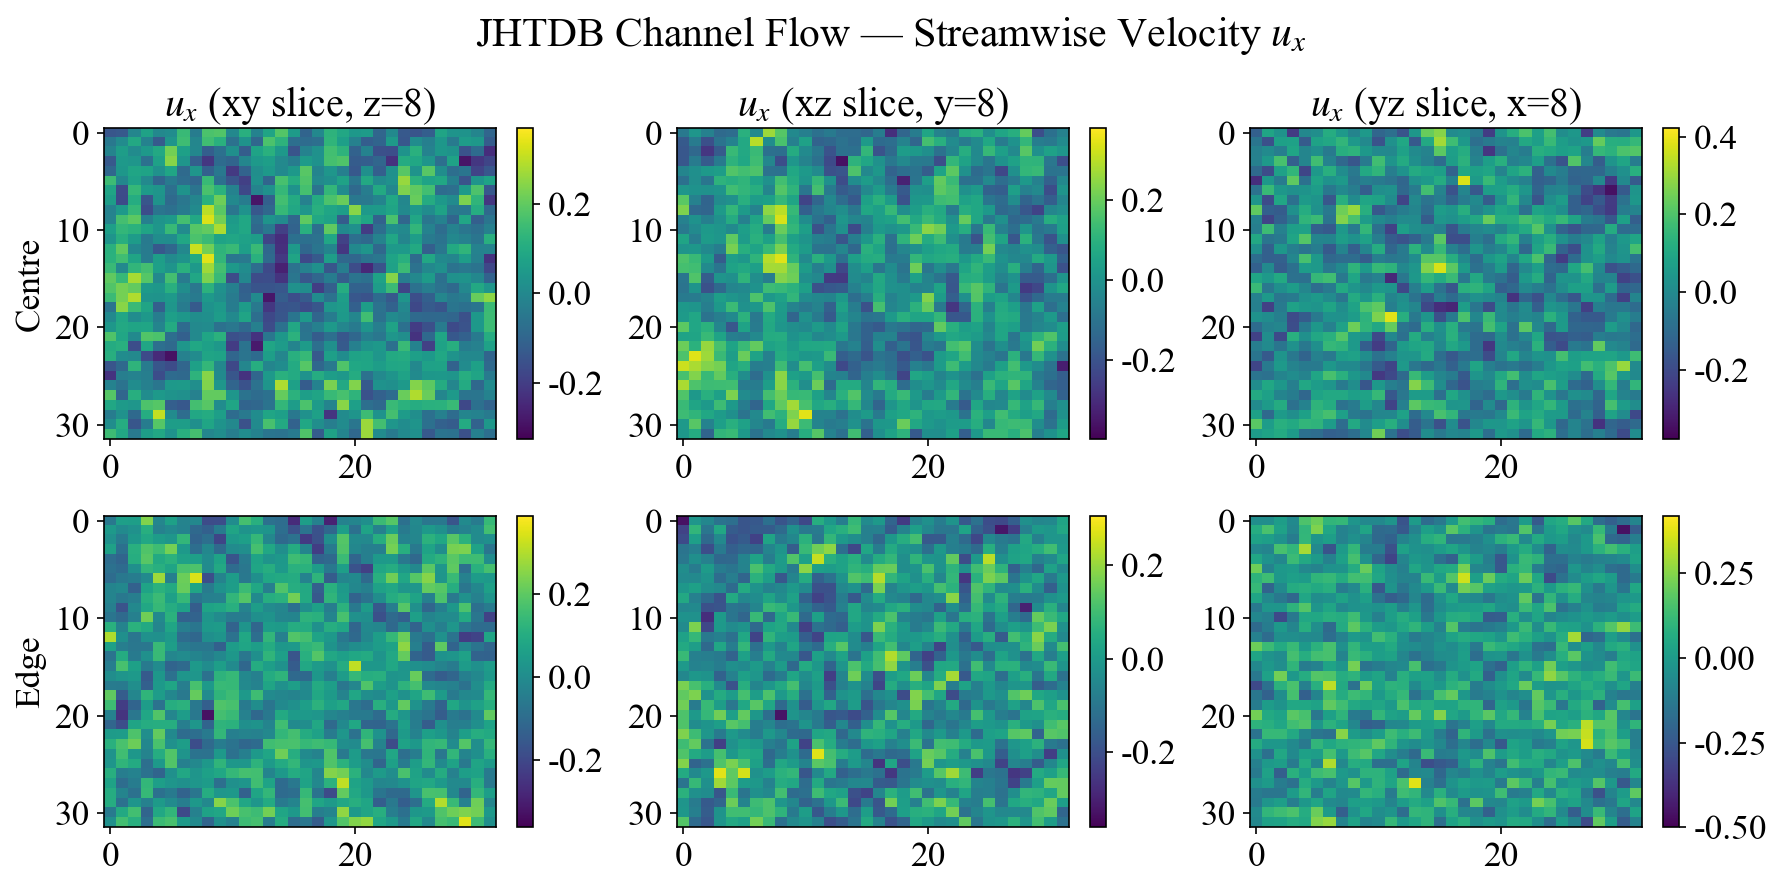
\includegraphics[width=0.9\textwidth]{figures/fig_data_samples.png}
\caption{Representative velocity-magnitude snapshots from the low-gradient ``centre'' group (left) and high-gradient ``edge'' group (right). The names are retained from the archived dataset and do not denote geometric centre/wall positions.}
\label{fig:data-samples}
\end{figure}

\textbf{Legacy synthetic noise protocol.} The superseded exploratory implementation corrupted fields with additive uniform noise:
\begin{equation}
\label{eq:noise-corruption}
f_\sigma(\mathbf{x}) = f(\mathbf{x}) + \sigma \, \xi_f(\mathbf{x}) \, s_f,
\end{equation}
where $f\in\{u_x,u_y,u_z,p\}$, $\sigma$ is the noise level, $\xi_f$ is i.i.d.\ uniform noise in $[-1,1]$, and $s_f$ is the empirical field standard deviation. The historical values were $\sigma\in\{0,0.1,0.5,1.0\}$; this protocol has not been rerun for the discovery-informed model.

\subsection{Experimental Setup}
\label{sec:setup}

\subsubsection{Baseline Methods}
\label{sec:baselines}

The formal matched comparison contains three variants:

\begin{itemize}
    \item \textbf{Local NoProp (none):} strictly local discrete NoProp with no physical loss.
    \item \textbf{Local NoProp (analytic):} the same model with prescribed continuity and the continuum pressure--Poisson coefficient $(1,1)$.
    \item \textbf{Discovery-informed NoProp (SPIDER):} the same model loading the held-out-validated terms and coefficients $(1,0.293)$ from the SPIDER artifact.
\end{itemize}

Legacy CNN, PINN, NoProp-CT, and post-hoc SPIDER-classifier results used a different split and are not included in the formal table.

\subsubsection{SPIDER-Discovered Equations}
\label{sec:discovered-equations}

The original broad-library implementation produced unstable zero-order and duplicate time-derivative relations and is retained only as legacy history. The corrected spatial SPIDER applies dimensional constraints before regression, uses all 80 archived snapshots in a 60/20 discovery/validation split, and recovers Eq.~\eqref{eq:discovered-pp}. Provenance is therefore:

\begin{itemize}
    \item \textbf{Continuity equation (prescribed by the incompressible DNS):}
    \begin{equation}
    \label{eq:continuity-discovered}
    \mathcal{R}_{\text{cont}}(\mathbf{u}) := \nabla\cdot\mathbf{u} = 0.
    \end{equation}
    
    \item \textbf{SPIDER-discovered spatial relation:}
    \begin{equation}
    \label{eq:pp-discovered}
    \mathcal{R}_{\text{SP}}(p,\mathbf{u}) := \nabla^2 p + 0.293\,\nabla\cdot[(\mathbf{u}\cdot\nabla)\mathbf{u}] = 0,
    \end{equation}
    selected from data and accepted only after held-out and bootstrap validation.
\end{itemize}

The analytic baseline uses the same structure with convection coefficient one. The difference between 0.293 and one is not hidden: it exposes the effective amplitude convention introduced by the archived generator's unscaled $3/2$ Fourier padding. Full forced Navier--Stokes recovery is not claimed because instantaneous forcing was not saved.

For reference, the DNS uses the known Navier--Stokes form with $\nu=5\times10^{-3}$:
\begin{equation}
\label{eq:ns-discovered}
\mathcal{R}_{\text{NS}}(\mathbf{u},p) := \partial_t\mathbf{u} + (\mathbf{u}\cdot\nabla)\mathbf{u} + \nabla p - \nu\nabla^2\mathbf{u} = 0,
\end{equation}
but the optimized single-snapshot training objective does not insert a duplicated artificial time axis and does not evaluate this full temporal residual.

\begin{figure}[htbp]
\centering
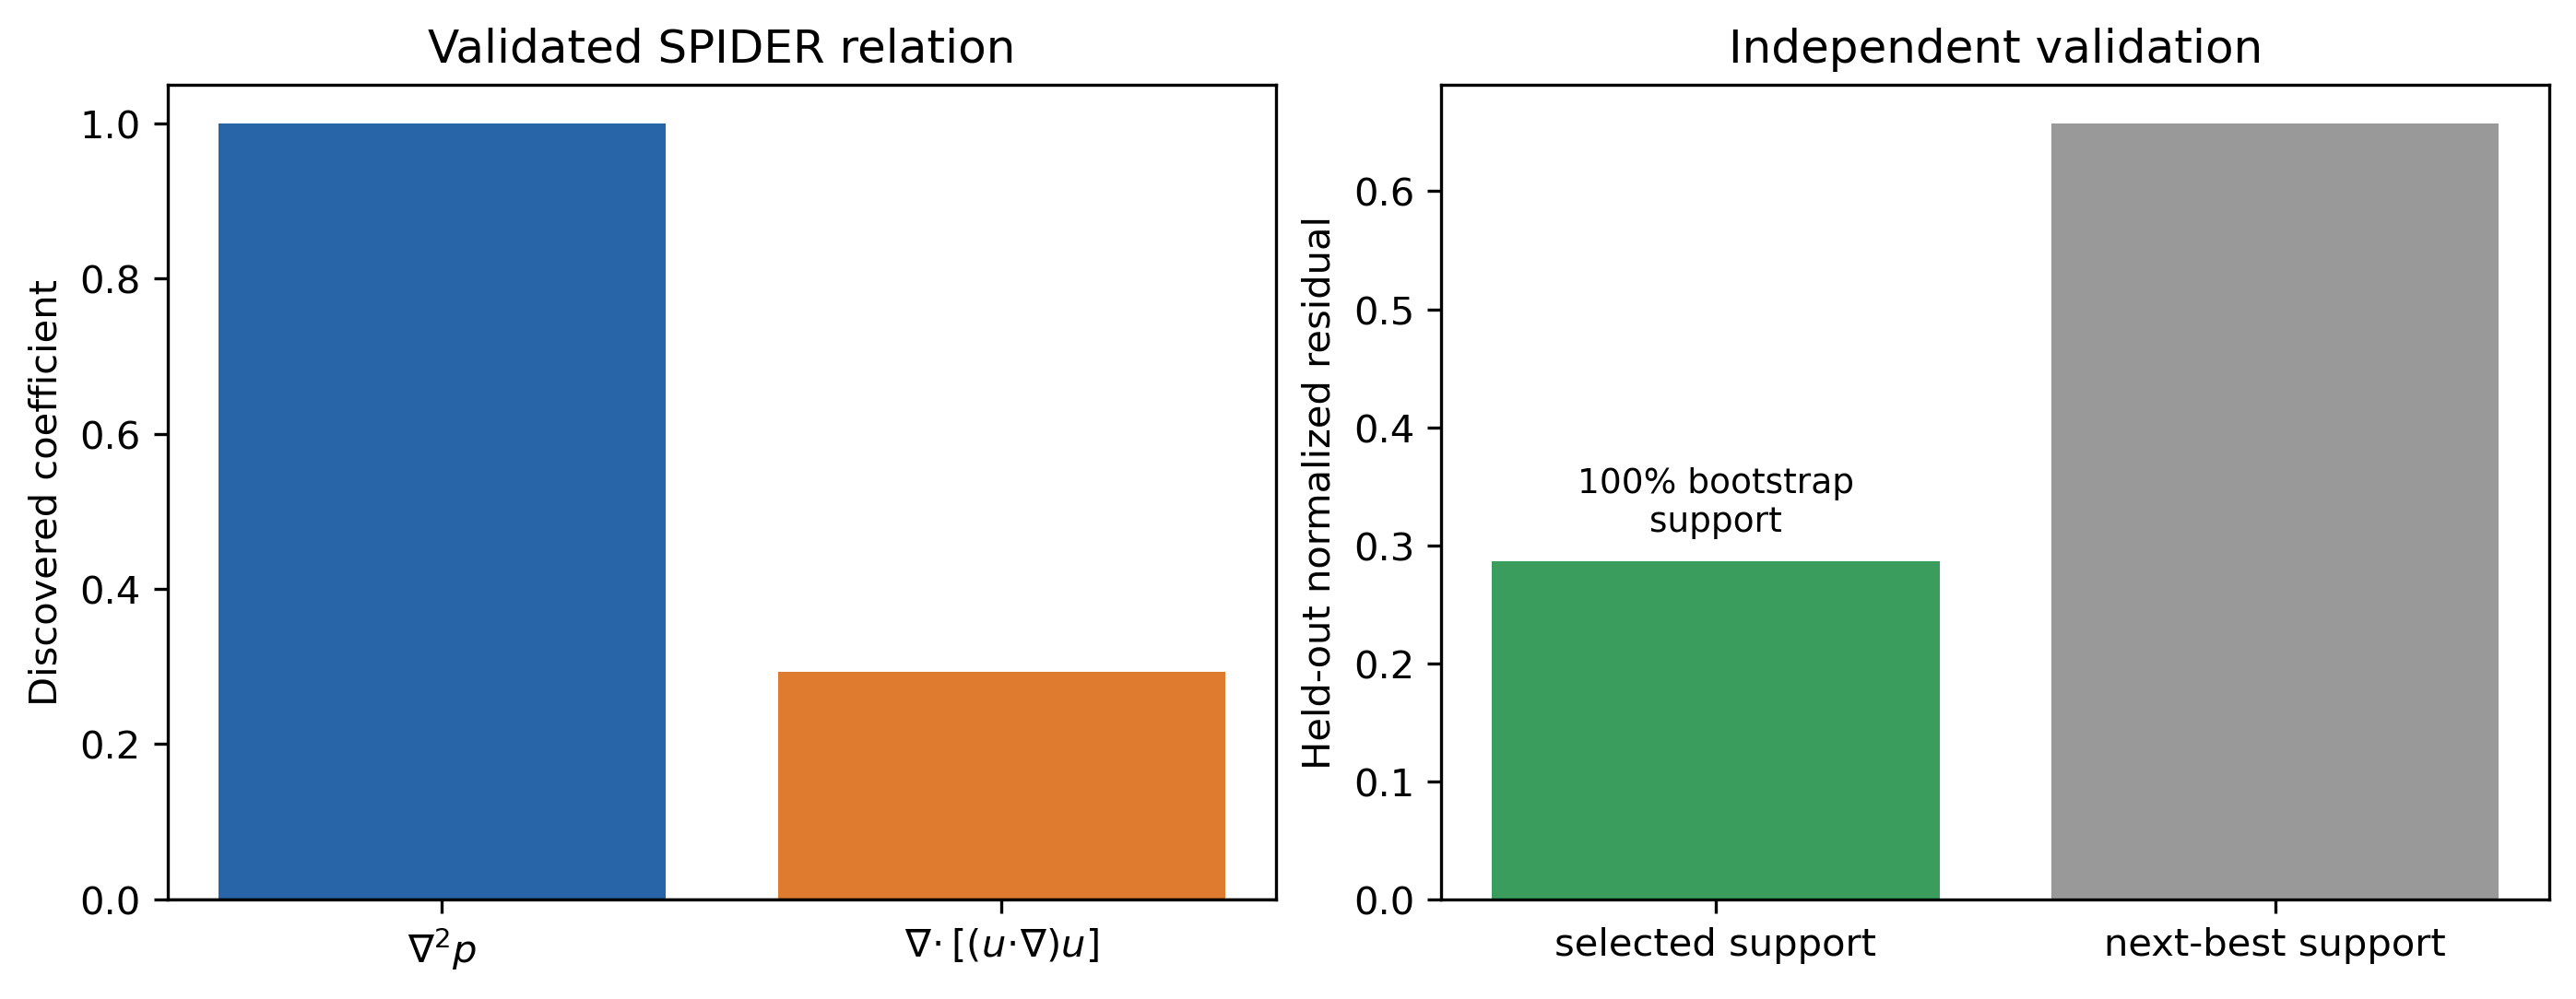
\includegraphics[width=\textwidth]{figures/fig_spider_discovery.png}
\caption{Validated spatial SPIDER result. Left: discovered coefficients after fixing the pressure-Laplacian coefficient to one. Right: held-out residual of the selected support and the next-best support; the selected support appears in all 100 bootstrap refits.}
\label{fig:spider}
\end{figure}

The resulting JSON artifact is read by the optimized trainer. Unit tests verify coefficient transfer, while any artifact with failed validation or unsupported terms raises an error.

\subsubsection{Implementation Details for PI-NoProp}
\label{sec:implementation-details}

\textbf{Network architecture.} The condition encoder adaptively pools the four input channels (three velocities and pressure) to $4^3$, followed by two fully connected layers producing a normalised 128-dimensional feature. Each of $T=10$ NoProp blocks is a three-hidden-layer MLP receiving the concatenated noisy latent and frozen condition feature. A compact transposed-convolution decoder maps a latent to the central $4\times16^3$ physical integration domain. Encoder-feature class centroids define the frozen target embeddings, aligning the diffusion target space with the decoder's autoencoding space.

\textbf{Training details.} The optimized path uses AdamW, learning rate $10^{-3}$, weight decay $10^{-4}$, batch size 64, automatic mixed precision, and TF32 on an 8\,GB RTX~4060 Laptop GPU. The encoder and compact decoder are pretrained once and frozen. At every local step, one block index $t$ is sampled and only that block's optimizer is updated; the objective is multiplied by $T$, providing an unbiased estimator of the sum over blocks. Each block receives 100 updates in the reported efficiency experiments. The classifier is trained afterward on detached final latents for 30 epochs. Eight deterministic compact-support test functions with $\beta=8$ are evaluated over $16^3$. Weak residual accumulation and normalisation are performed in FP32.

\textbf{Comparison protocol.} The formal comparison uses identical frozen shared components and fixed 192/32/32 train/validation/test splits for no physics, analytic physics, and SPIDER-discovered physics. Results are aggregated over seeds $\{0,1,2\}$. Every checkpoint is evaluated with both coefficient sets; Table~\ref{tab:main-results} uses the SPIDER residual as a common ruler for all methods.

\begin{figure}[htbp]
\centering
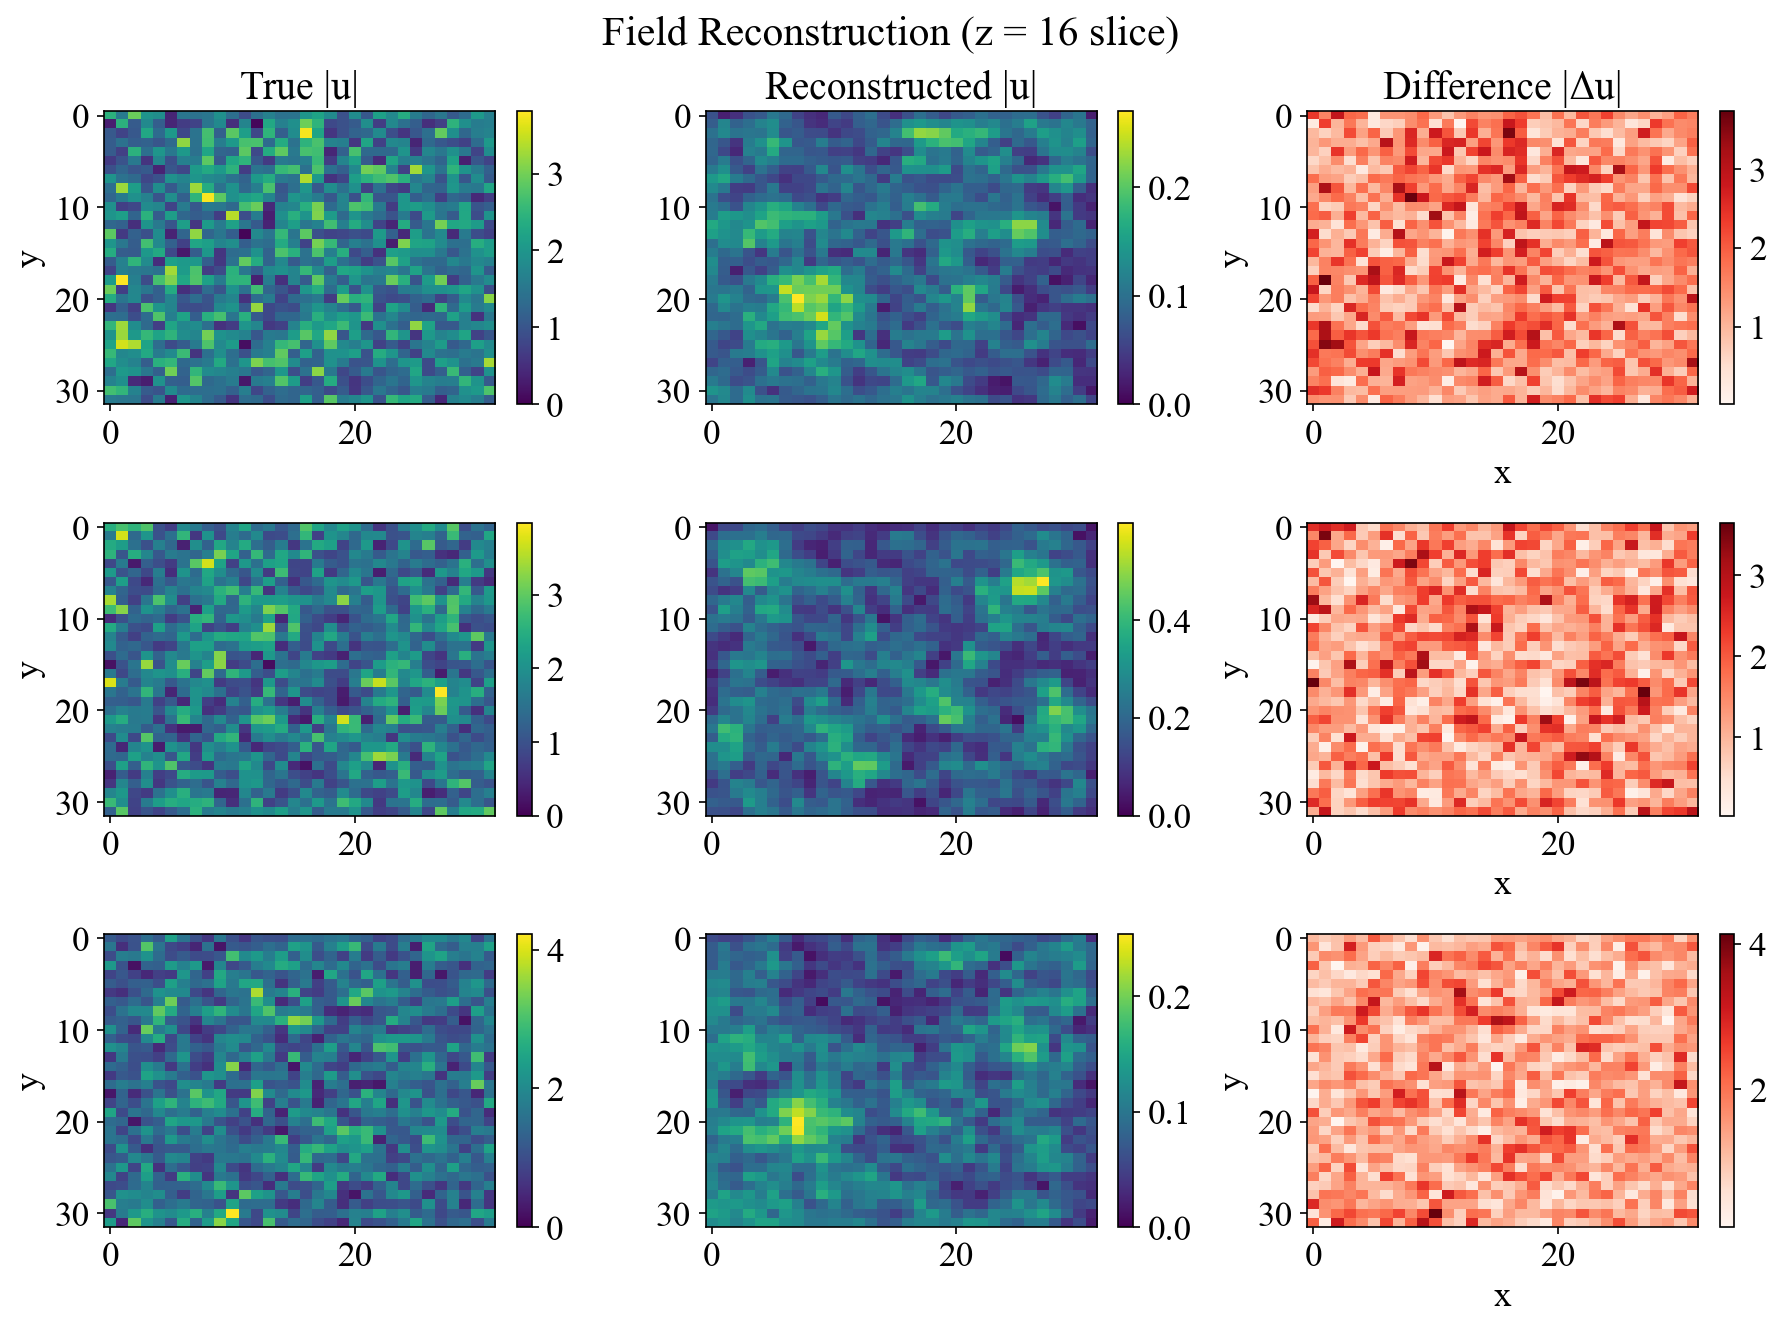
\includegraphics[width=0.48\textwidth]{figures/fig_field_reconstruction_centre.png}
\hfill
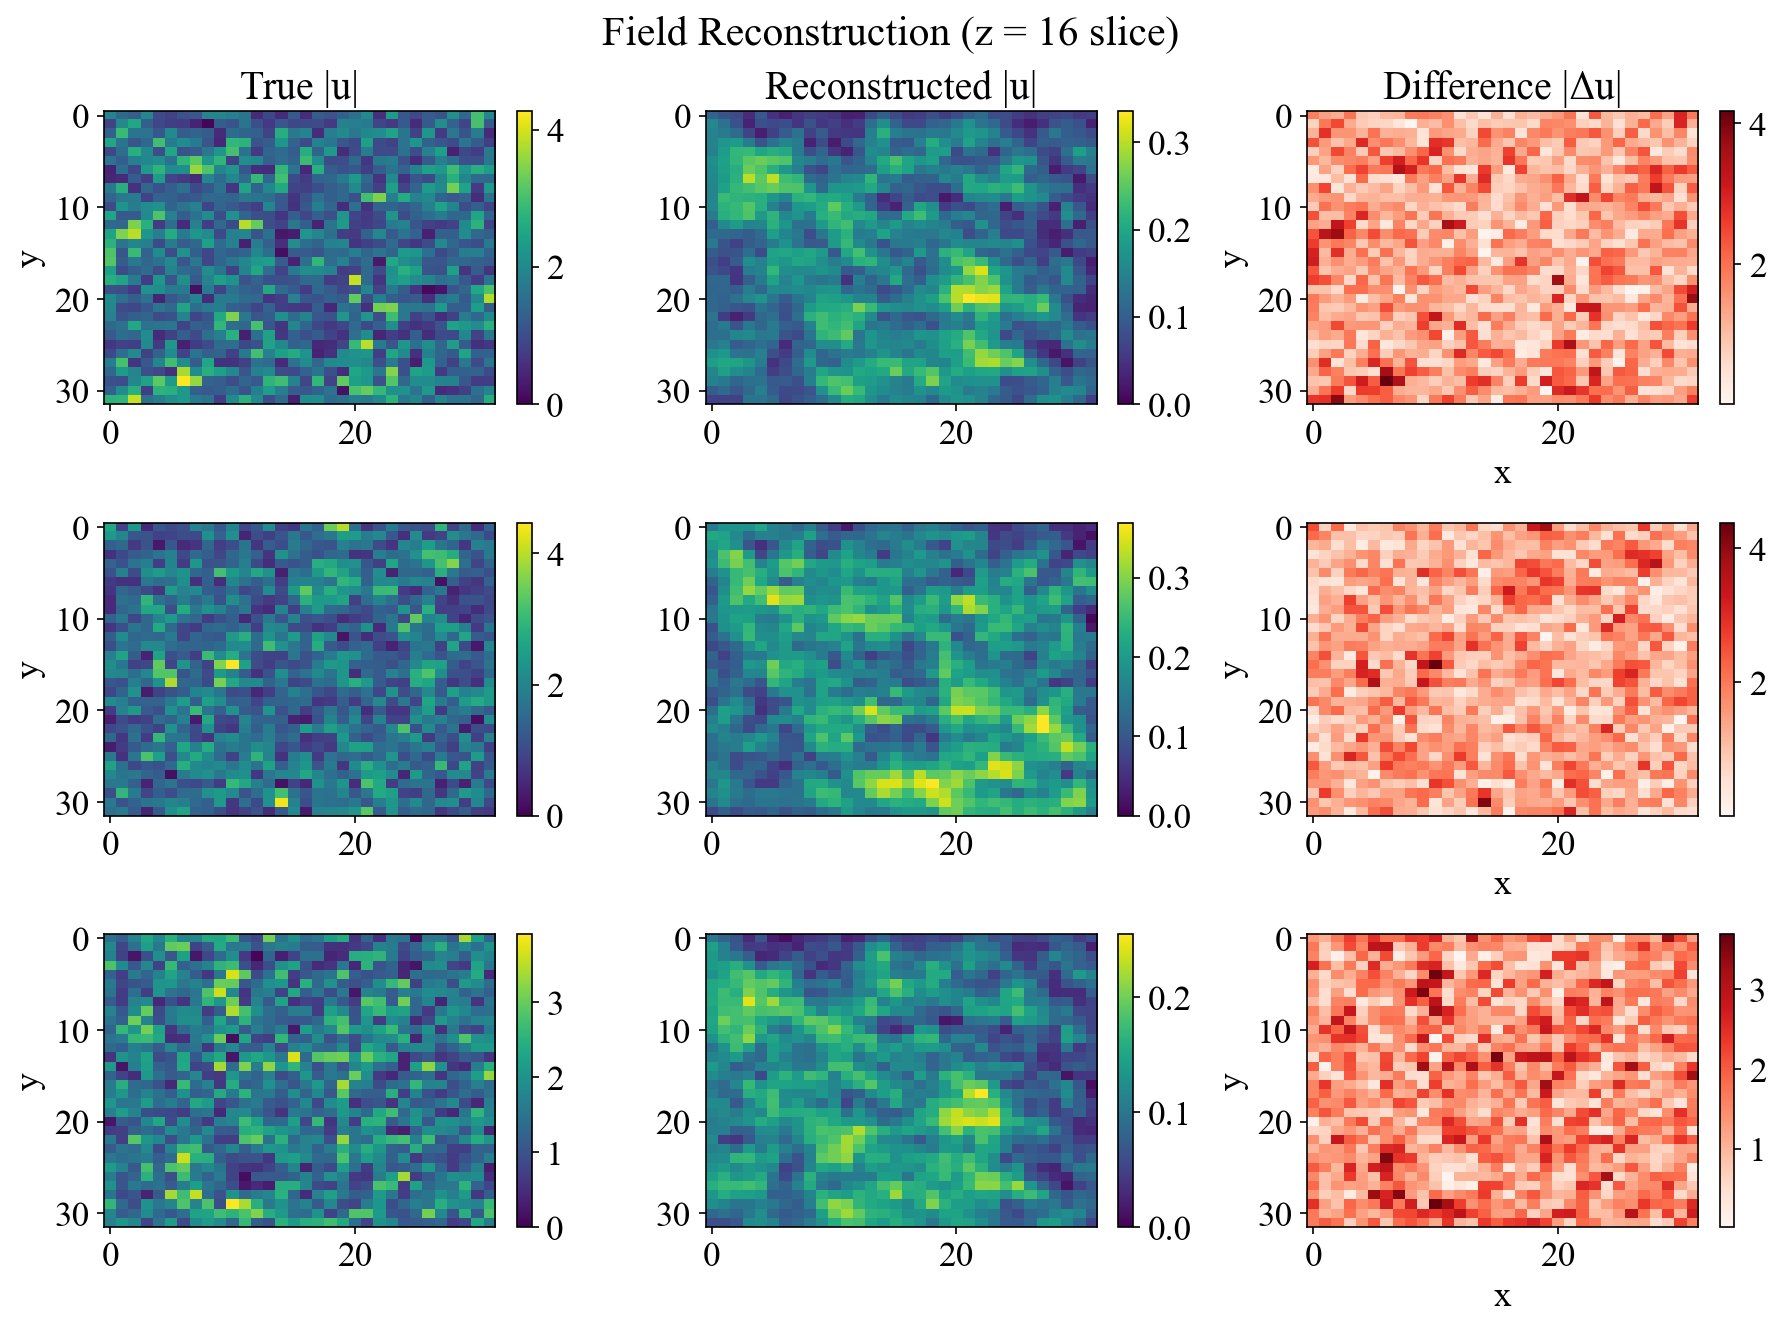
\includegraphics[width=0.48\textwidth]{figures/fig_field_reconstruction_edge.png}
\caption{Legacy decoder reconstruction examples for the centre (left) and edge (right) groups. Each panel shows original and reconstructed $u_x$ slices. These examples are qualitative and are not used to establish decoder fidelity for the optimized checkpoints.}
\label{fig:field-reconstruction}
\end{figure}

\textbf{Evaluation metrics.} We report:

\begin{itemize}
    \item \textbf{Classification accuracy} (top-1) on the test set.
    \item \textbf{Consistency residuals:} dimensionless continuity and discovered-relation weak residuals. For weak contributions $q_j$,
    \begin{equation}
    \label{eq:relative-residual}
    \eta = \operatorname{RMS}_{k}\left(\frac{\sum_j q_{j,k}}{\sum_j|q_{j,k}|+\epsilon}\right).
    \end{equation}
    Lower $\eta_{\mathrm{div}}$ and $\eta_{\mathrm{SP}}$ indicate better adherence to the prescribed continuity and discovered relation, respectively.
    \item \textbf{Computational efficiency:} complete local block-phase time and peak GPU memory.
\end{itemize}

\subsection{Main Results: Classification Accuracy and Physical Consistency}
\label{sec:main-results}

Table~\ref{tab:main-results} presents held-out test accuracy and dimensionless spatial weak residuals under the optimized local protocol. Values are aggregated over seeds $\{0,1,2\}$; each test split contains 32 samples, so one prediction changes accuracy by 3.125 percentage points.

\begin{table}[htbp]
\centering
\caption{Discovery-to-training results (mean $\pm$ standard deviation over three seeds). Every method is evaluated with the same SPIDER coefficient for $\eta_{\mathrm{SP}}$.}
\label{tab:main-results}
\resizebox{\textwidth}{!}{%
\begin{tabular}{lcccccc}
\toprule
Method & \multicolumn{3}{c}{Centre} & \multicolumn{3}{c}{Edge} \\
\cmidrule(lr){2-4} \cmidrule(lr){5-7}
& Accuracy $\uparrow$ & $\eta_{\mathrm{div}}\downarrow$ & $\eta_{\mathrm{SP}}\downarrow$
& Accuracy $\uparrow$ & $\eta_{\mathrm{div}}\downarrow$ & $\eta_{\mathrm{SP}}\downarrow$ \\
\midrule
Local NoProp (none) & $33.33\pm6.51$ & 0.420 & 0.293 & $27.08\pm3.61$ & 0.413 & 0.244 \\
Local NoProp (analytic) & $33.33\pm6.51$ & 0.171 & 0.213 & $25.00\pm0.00$ & \textbf{0.107} & 0.179 \\
Discovery-informed NoProp (SPIDER) & $33.33\pm3.61$ & \textbf{0.124} & \textbf{0.158} & $27.08\pm4.77$ & 0.110 & \textbf{0.145} \\
\bottomrule
\end{tabular}
}
\end{table}

The optimized results support three conclusions:

\begin{itemize}
    \item \textbf{No resolved accuracy gain is observed.} The discovered model matches vanilla NoProp's mean accuracy in both groups; the overlapping-crop split, small test set, and seed variation do not support a predictive-improvement claim.
    \item \textbf{The discovered artifact is operational, not post-hoc.} Training with its coefficients reduces the common SPIDER residual from 0.293 to 0.158 in the centre and from 0.244 to 0.145 at the edge. It also gives the lowest centre continuity residual.
    \item \textbf{Discovery and analytic priors are empirically distinct.} The discovered coefficient improves the metric it was selected to represent more than the continuum coefficient, while the analytic prior obtains the lowest edge continuity residual. Reporting both avoids conflating prescribed and learned physics.
    \item \textbf{The high-gradient edge group remains harder.} All variants obtain lower edge accuracy under the internal split, consistent with its larger velocity-gradient proxy and weak mean-velocity label.
\end{itemize}

These results replace the earlier single-seed validation-only table. Legacy results are not directly comparable because they did not reserve a test set and used joint cross-block back-propagation.

\begin{figure}[htbp]
\centering
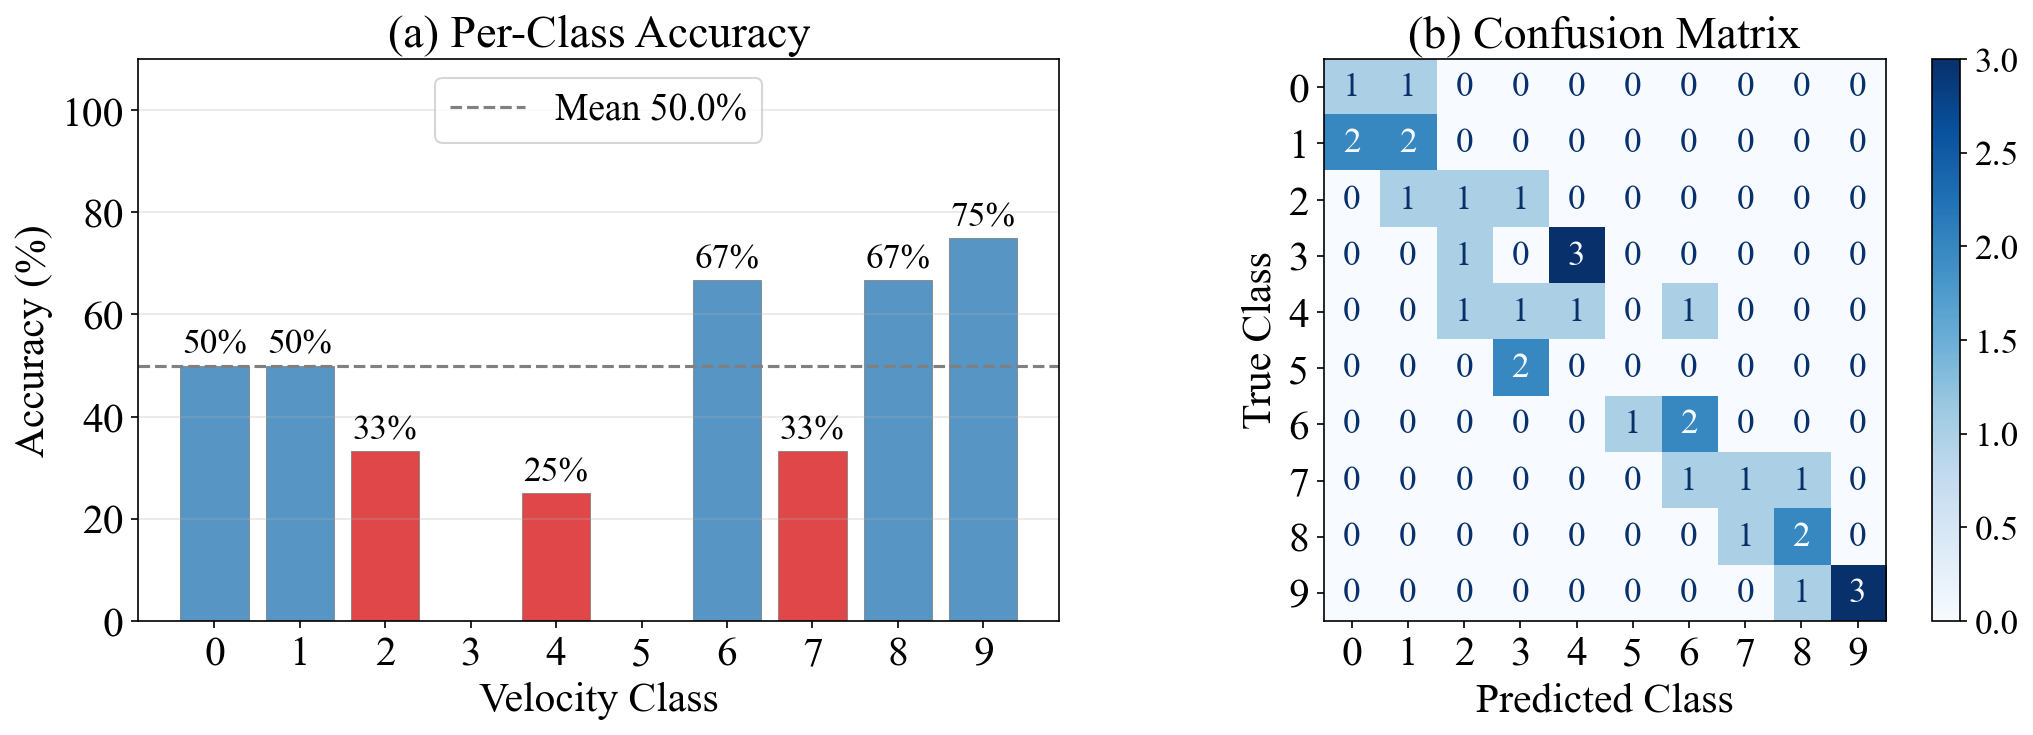
\includegraphics[width=0.8\textwidth]{figures/fig_region_comparison.png}
\caption{Legacy single-seed validation comparison retained for historical context. It uses the former joint-training protocol and must not be compared numerically with Table~\ref{tab:main-results}.}
\label{fig:region-comparison}
\end{figure}

\begin{figure}[htbp]
\centering
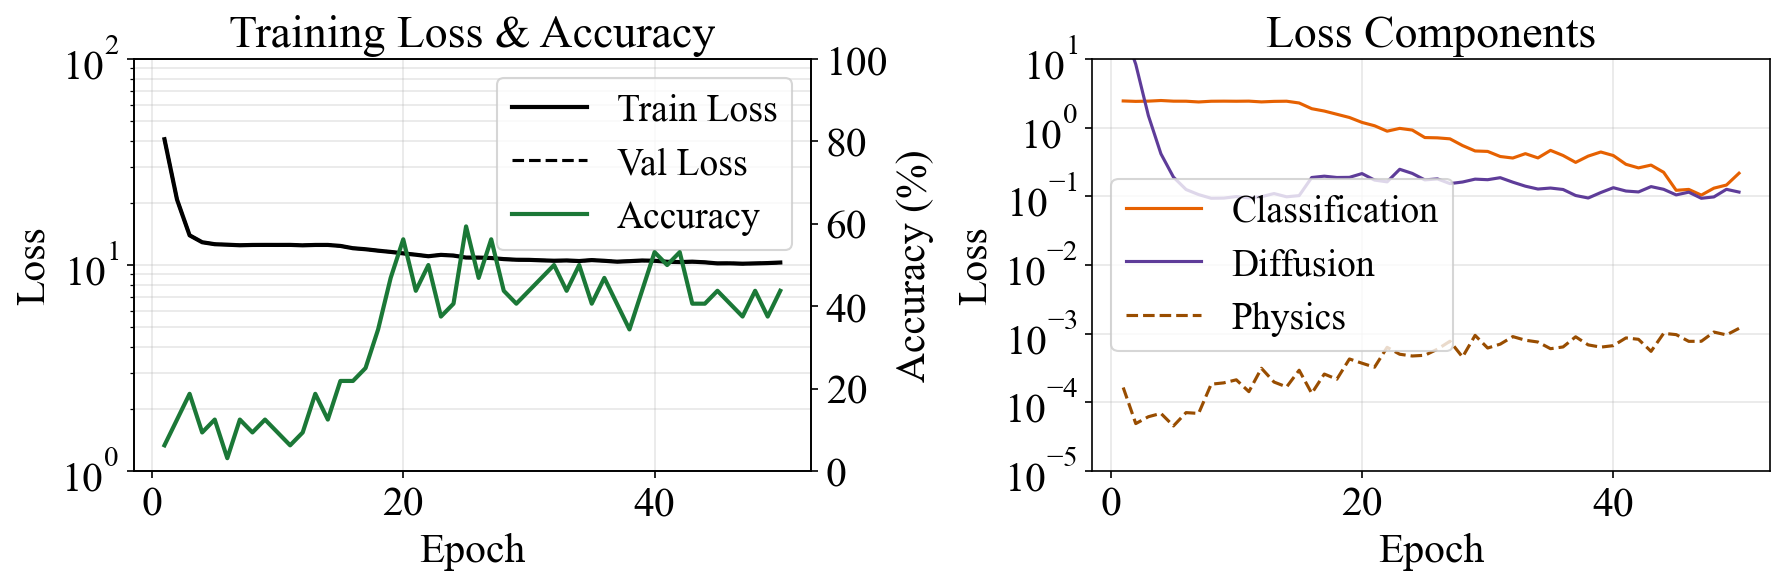
\includegraphics[width=0.85\textwidth]{figures/fig_training_curves.png}
\caption{Legacy joint-training curves. Optimized local runs are recorded by block update rather than a joint epoch and are stored separately under \texttt{outputs/runs}.}
\label{fig:training-curves}
\end{figure}

\subsection{Robustness to Noise}
\label{sec:noise-robustness}

Figure~\ref{fig:noise-robustness} records an exploratory noise sweep from the legacy joint-training implementation. It is retained to document project history but is not evidence for the optimized strictly local method; a matched multi-seed noise sweep remains future work.

\begin{figure}[htbp]
\centering
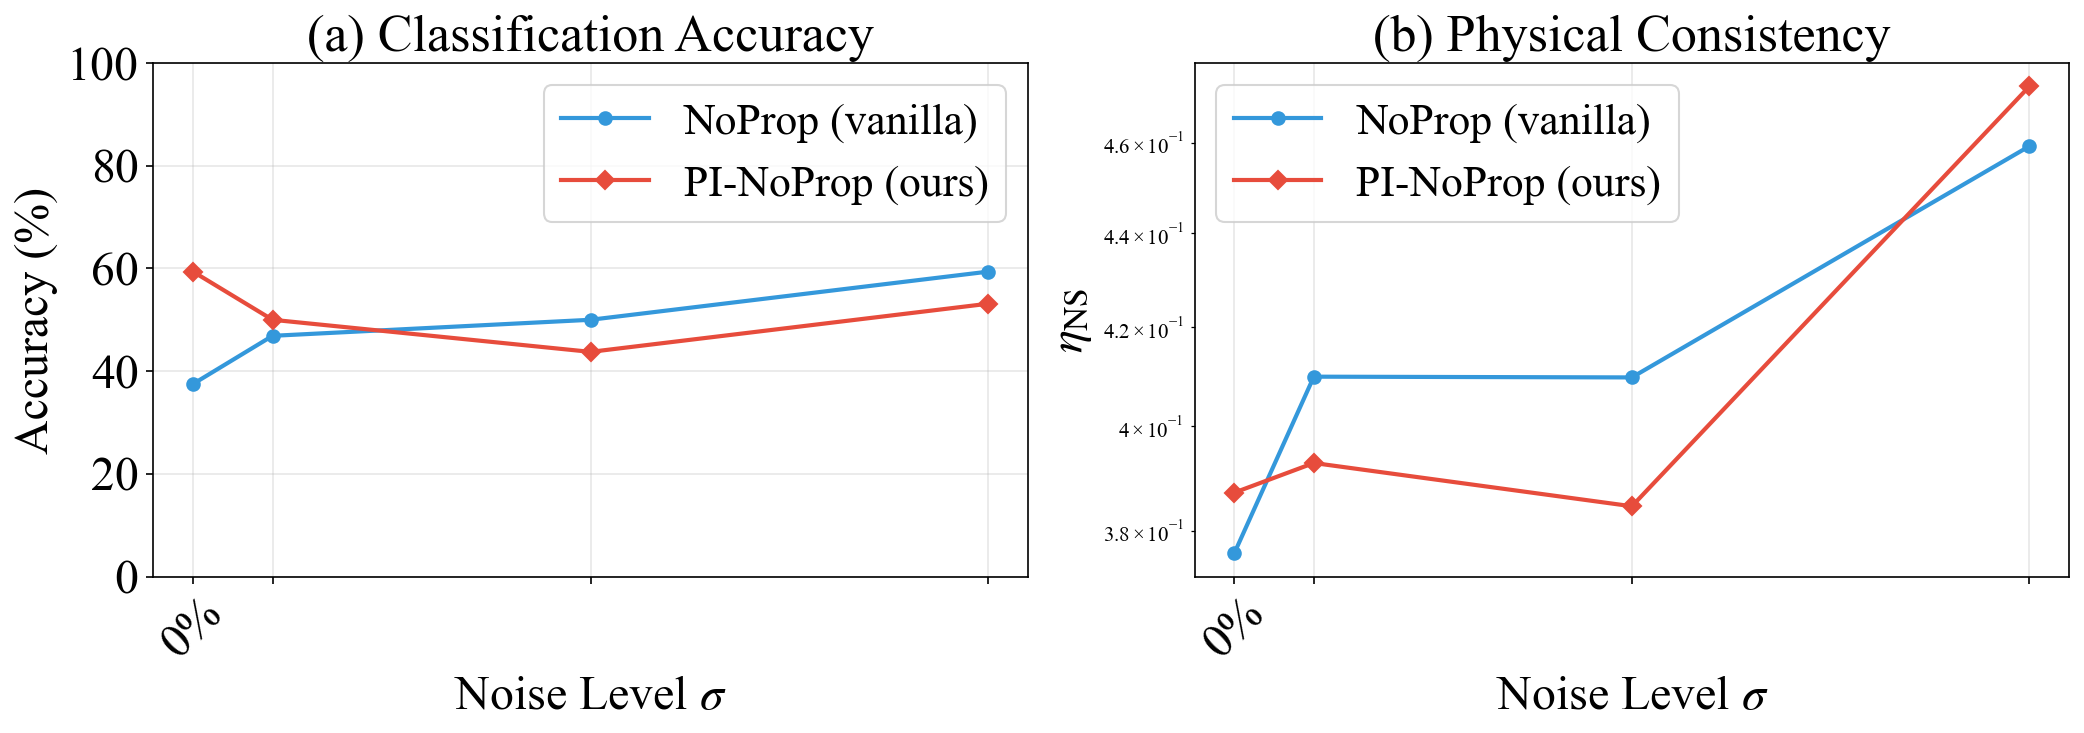
\includegraphics[width=\textwidth]{figures/fig_noise_robustness.png}
\caption{Legacy single-run noise sweep from the superseded joint-training implementation. It is shown only as project history and does not support claims about the discovery-informed model.}
\label{fig:noise-robustness}
\end{figure}

Because this sweep used a different split, a temporal residual constructed from replicated snapshots, and cross-block joint optimisation, no pointwise interpretation is transferred to the present method. A matched three-seed noise study remains future work.

\subsection{Ablation Studies}
\label{sec:ablations}

\subsubsection{Influence of the Physics Loss Weight}
\label{sec:lambda-ablation}

We repeat the $\lambda$ sweep using the validated SPIDER artifact, the optimized dimensionless spatial loss, the fixed held-out split, and seeds $\{0,1,2\}$.

\begin{figure}[htbp]
\centering
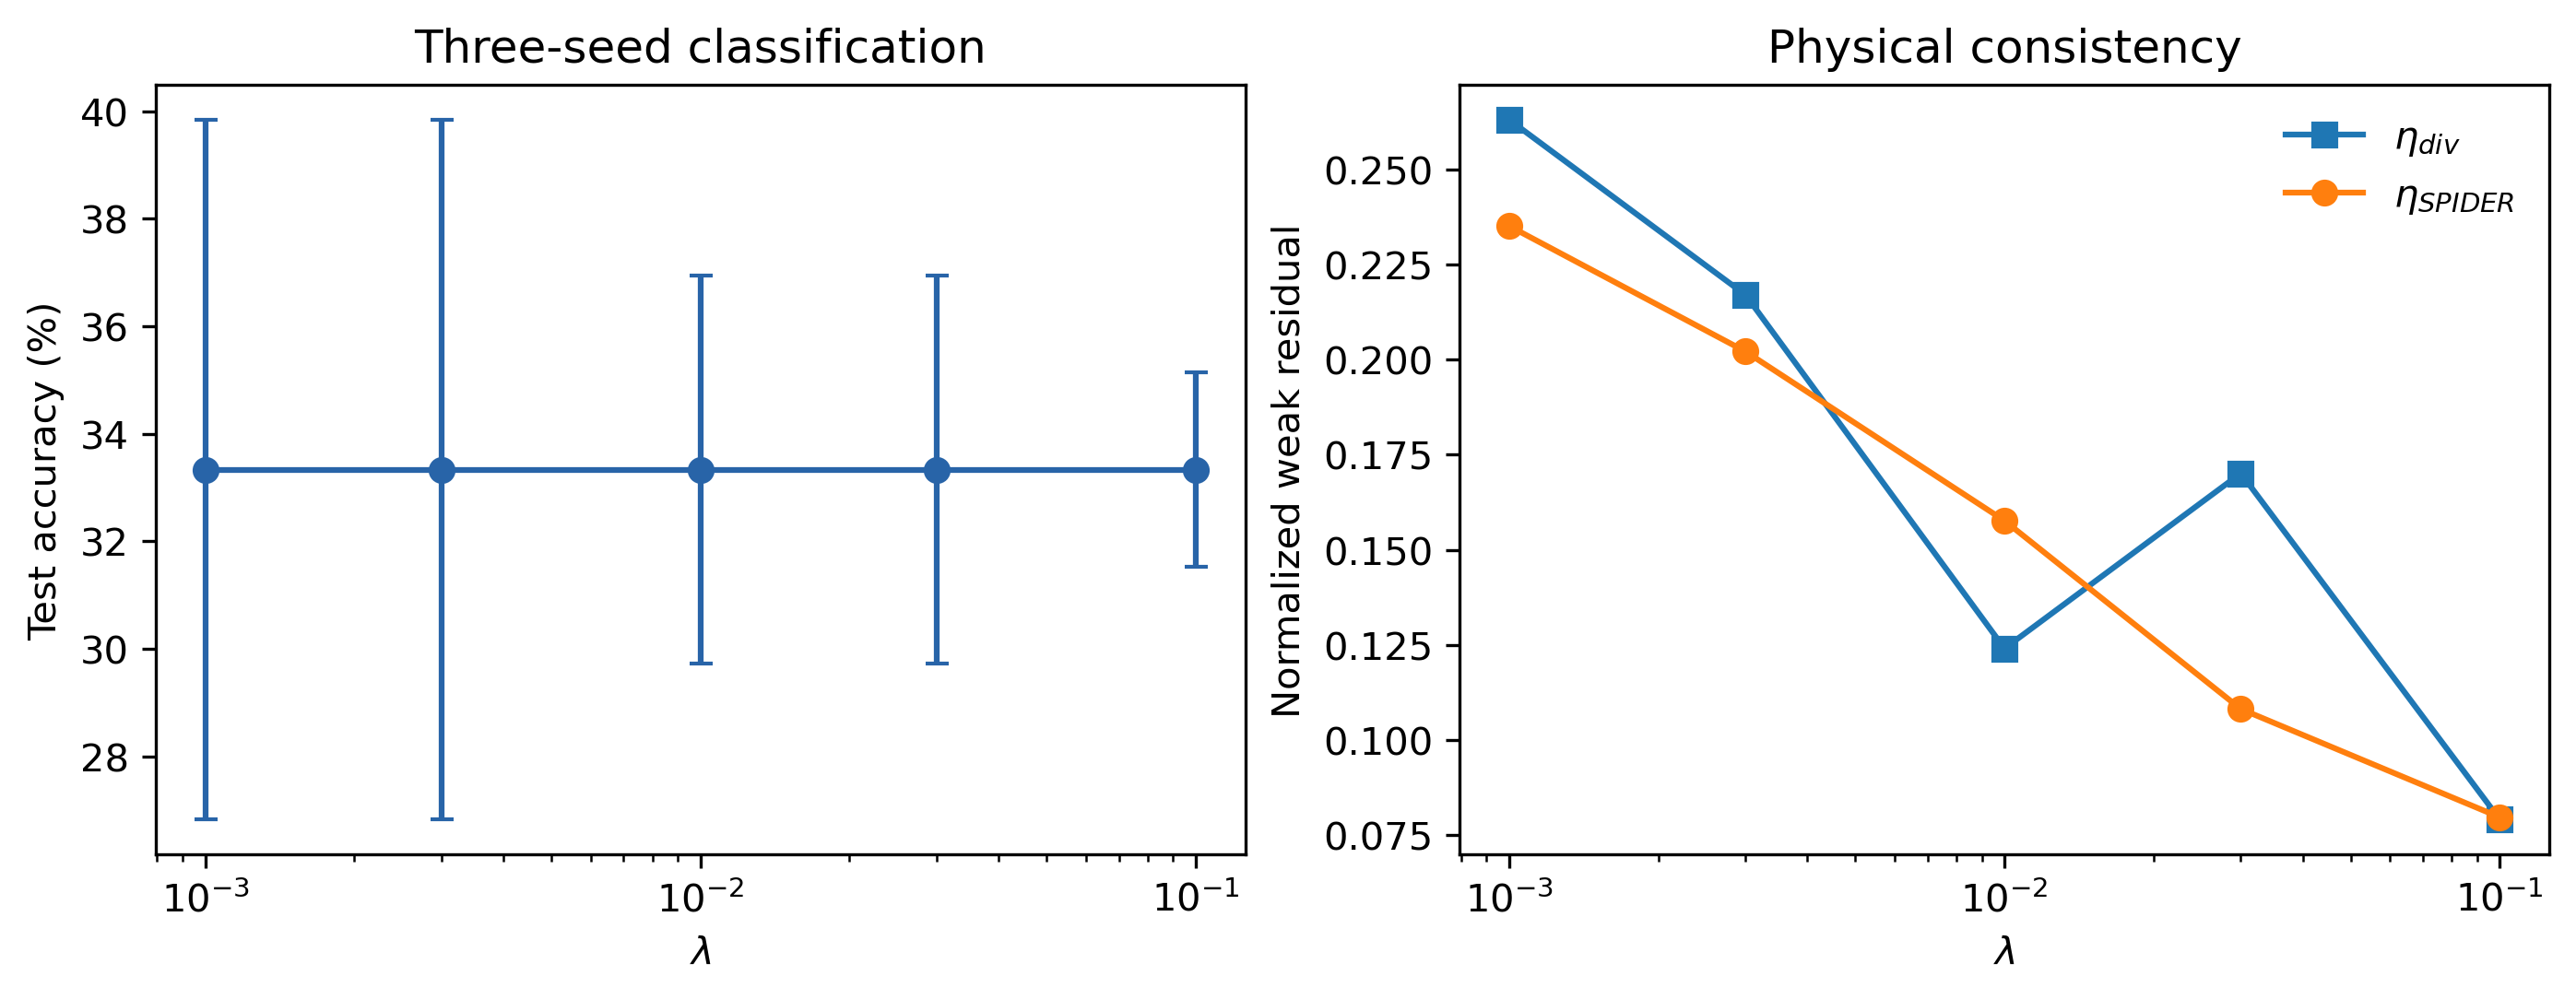
\includegraphics[width=\textwidth]{figures/fig_lambda_tradeoff.png}
\caption{Matched three-seed sweep for discovery-informed NoProp on the centre test split. Accuracy is unchanged within the resolution of the 32-sample test set, while the discovered-equation residual decreases monotonically with $\lambda$.}
\label{fig:lambda-tradeoff}
\end{figure}

Mean accuracy is 33.33\% at every tested value; its across-seed standard deviation decreases from 6.51 points at $10^{-3}$ to 1.80 points at $10^{-1}$. In contrast, $\eta_{\mathrm{SP}}$ decreases from 0.235 to 0.080. Thus $\lambda$ controls physical adherence but does not rescue the weak classification label. We retain $10^{-2}$ for the main table as a moderate setting rather than choosing $10^{-1}$ after inspecting the test residual.

\subsubsection{Choice of Discovered Equations}
\label{sec:equation-ablation}

Table~\ref{tab:main-results} is the equation-source ablation: no equation, an analytically prescribed coefficient, and the SPIDER-discovered coefficient. All three use the same architecture, split, seeds, and update count. This directly tests whether discovery changes training, rather than comparing unrelated legacy temporal losses.

\subsubsection{Effect of Decoder Architecture}
\label{sec:decoder-ablation}

The optimized decoder maps the 128-dimensional latent to a $4\times16\times16\times16$ field and is frozen after feature-conditioned reconstruction pretraining. A dedicated architecture sweep has not been performed; accordingly, decoder expressiveness remains a limitation rather than an indirectly ``confirmed'' property.

\subsection{Analysis of Learned Latent Representations}
\label{sec:representation-analysis}

Figure~\ref{fig:tsne} is a legacy single-run t-SNE visualisation. It is retained as qualitative project history and has not yet been regenerated for the optimized three-seed checkpoints.

\begin{figure}[htbp]
\centering
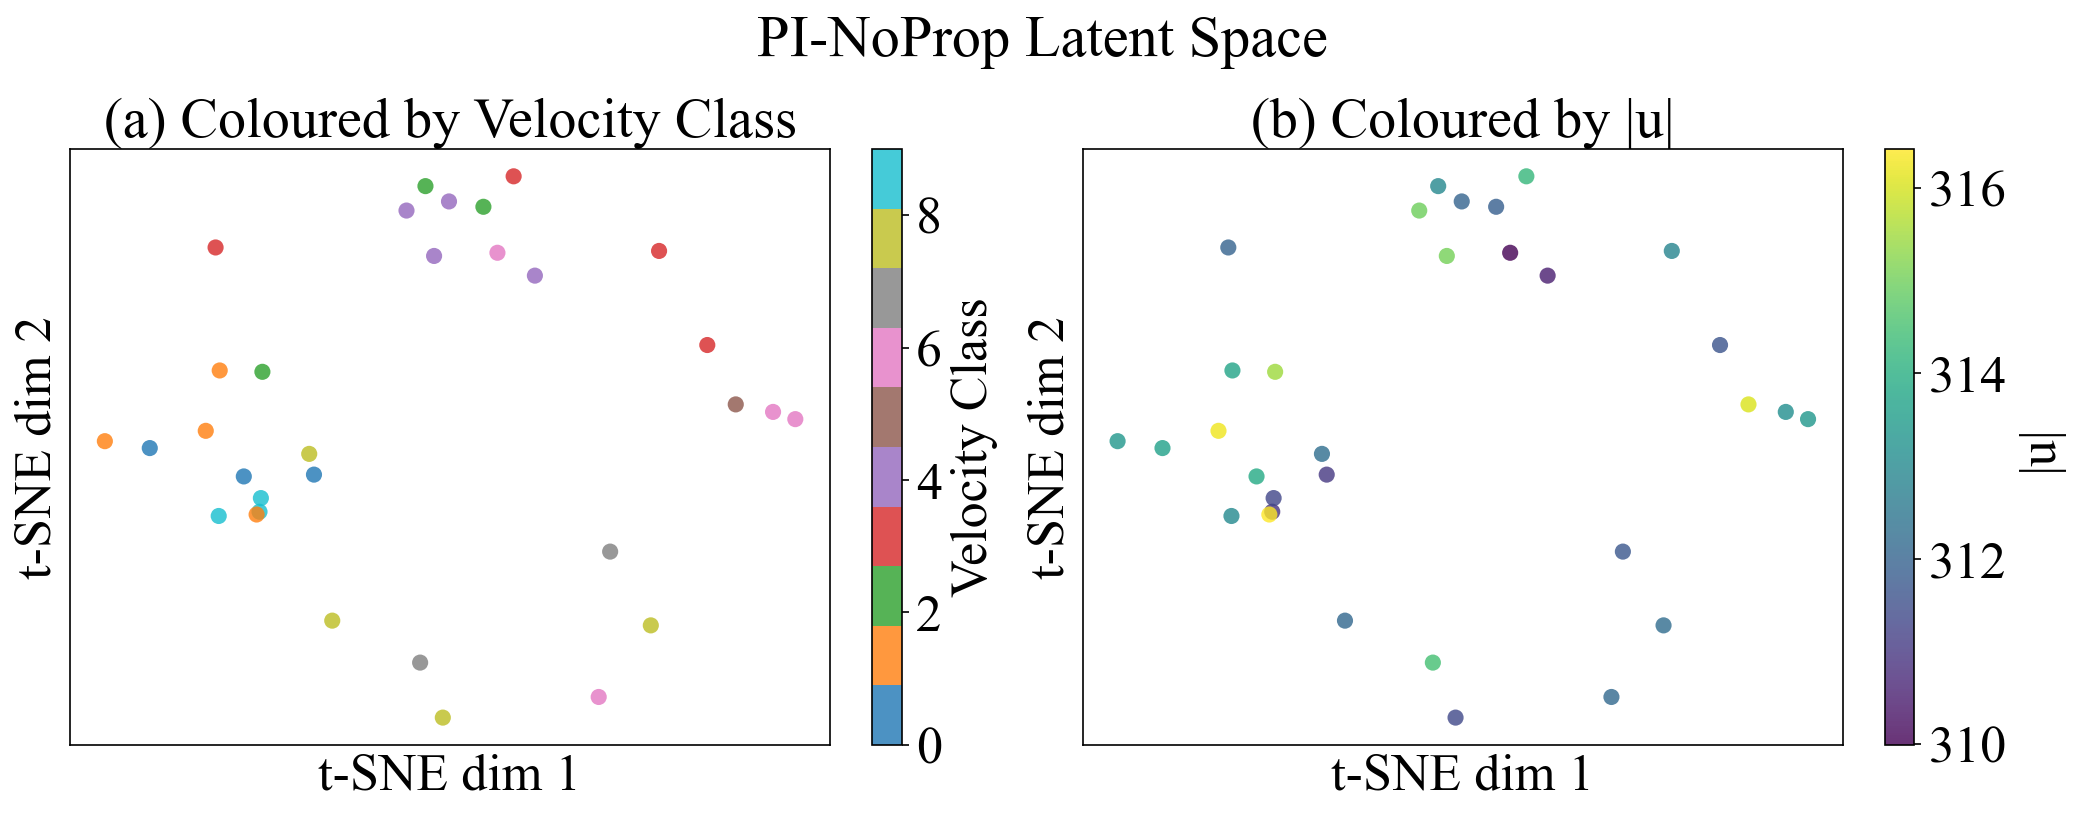
\includegraphics[width=0.8\textwidth]{figures/fig_tsne.png}
\caption{Legacy t-SNE visualisation from the superseded joint-training run. It is not evidence for the optimized discovery-informed checkpoints.}
\label{fig:tsne}
\end{figure}

Because t-SNE is stochastic and this figure comes from the former joint-training protocol, it is not used as confirmatory evidence in the revised conclusions.

\subsection{Computational Efficiency}
\label{sec:efficiency}

Table~\ref{tab:efficiency} reports the measured complete local block-training phase on an NVIDIA RTX~4060 Laptop GPU (8\,GB), averaged over the three official seeds. Shared encoder/decoder pretraining and subsequent classifier training are excluded.

\begin{table}[htbp]
\centering
\caption{Optimized local block-training efficiency (100 updates per block).}
\label{tab:efficiency}
\resizebox{\textwidth}{!}{%
\begin{tabular}{lccc}
\toprule
Method & Centre time (s) & Edge time (s) & Peak GPU memory (MB) \\
\midrule
Local NoProp (none) & 6.3 & 6.4 & 286 \\
Local NoProp (analytic) & 14.4 & 14.6 & 499 \\
Discovery-informed NoProp (SPIDER) & 14.7 & 14.6 & 499 \\
\bottomrule
\end{tabular}
}
\end{table}

\begin{itemize}
    \item One uniformly sampled block is updated per step; all ten blocks receive exactly 100 updates, and no cross-block graph is retained.
    \item The physics path approximately doubles local block time but remains below 15 seconds per formal run; vanilla local training is approximately 6.3 seconds.
    \item The complete clean regional dataset (128 MB), model, and optimizer state fit comfortably on the 8 GB GPU. The measured peak is below 0.5 GB for the optimized block phase.
    \item A microbenchmark shows a 4--5.3$\times$ speed-up for the spatial weak loss relative to the legacy duplicated-time loss. First-frame caching also eliminates repeated decompression of approximately 7.4 GB of trajectory NPZ files.
\end{itemize}

\subsection{Discussion}
\label{sec:discussion}

The optimized experiments support a narrower set of conclusions than the original single-run study:

\begin{enumerate}
    \item \textbf{Strict locality is achieved:} each block has an independent optimizer, and automated tests verify that non-selected blocks, the frozen encoder, and the frozen decoder receive no gradients.
    \item \textbf{The discovery-to-training chain is achieved:} a held-out-validated SPIDER artifact is loaded by every local block, and its coefficient transfer is covered by automated tests.
    \item \textbf{Physical residuals improve:} the discovered model consistently lowers its common SPIDER residual in both regions and gives the lowest centre continuity residual.
    \item \textbf{Accuracy improvement is not established:} the three-seed means do not improve over vanilla local NoProp. Because crops overlap across index splits, stronger predictive claims require a trajectory- or space-grouped dataset in addition to more samples or a better physical label.
    \item \textbf{Training is practical:} first-frame/GPU caching, sampled blocks, mixed precision, and spatial weak forms reduce repeated local training to seconds rather than the legacy 10--20 minute joint runs.
\end{enumerate}

\textbf{The HIT versus channel flow trade-off.} We deliberately chose HIT over the more conventional channel flow benchmark used in \cite{gurevich2024learning}. While channel flow provides natural class separation via the mean velocity profile (centre $\approx$ fast, wall $\approx$ slow), it requires computationally expensive DNS (e.g., $2048\times512\times1536\times4000$ grid) that is inaccessible without supercomputing resources. HIT, solvable at $64^3$ resolution on a single consumer GPU, makes the full experimental pipeline reproducible. The cost is a substantially harder classification task: HIT's statistical homogeneity means that $\langle u_x \rangle \approx 0$ for all subdomains, compressing the class bins into a narrow range. We view this as a strength rather than a weakness: it provides a \textit{stress test} for the physics loss. If PI-NoProp can improve accuracy when the data signal is near the noise floor, it should generalise well to richer datasets where the physics constraint acts in concert with, rather than in lieu of, informative features.

Limitations include: (i) SPIDER recovers a validated spatial pressure relation but not the full forced momentum equation; (ii) the effective coefficient reflects the archived solver's padding convention; (iii) prescribed continuity accompanies the discovered relation; (iv) the $16^3$ integration domain may miss fine-scale violations; and (v) each 32-sample validation/test split has a coarse 3.125 percentage-point resolution.



\section{Conclusion}
\label{sec:conclusion}

We have presented a strictly local discovery-informed NoProp implementation for single-snapshot HIT data. The method discovers a spatial relation from 60 DNS snapshots, validates it on 20 disjoint snapshots and 100 bootstrap refits, persists the result, and rejects unvalidated artifacts. The accepted terms and coefficients are then used directly by independently optimised NoProp blocks.

SPIDER selects $\nabla^2p+0.293\,\nabla\cdot[(\mathbf u\cdot\nabla)\mathbf u]=0$ with held-out residual 0.286, a 2.30-fold separation from the next support, and 100\% bootstrap support. Continuity is separately identified as prescribed. A frozen compact decoder maps each block latent to a physical integration field, on which dimensionless weak residuals are evaluated. The local physics loss has the form
\begin{equation}
\label{eq:physics-loss-conclusion}
\mathcal{L}_{\text{phys}}^{(t)} = \frac{1}{|\mathcal{K}|}\sum_{k\in\mathcal{K}} \left(|\eta_{t,k}^{\mathrm{div}}|^2+\tfrac12|\eta_{t,k}^{\mathrm{SP}}|^2\right).
\end{equation}
Only the sampled block receives the scaled local denoising-plus-physics objective; the classifier is optimised later on detached final latents. Thus the following expression is a conceptual sum, not a joint back-propagation graph:
\begin{equation}
\label{eq:total-loss-conclusion}
\mathcal{L}_{\mathrm{local}} = \sum_{t=1}^T \left(\mathcal L_{\mathrm{diff}}^{(t)}+\lambda\mathcal L_{\mathrm{phys}}^{(t)}\right).
\end{equation}

We evaluated the framework on the archived forced-HIT run at final $Re_\lambda=30.5$. The verified findings are:

\begin{itemize}
    \item The discovered model reduces the common SPIDER residual from 0.293 to 0.158 in the centre and from 0.244 to 0.145 at the edge.
    \item Three-seed test accuracy does not show a statistically reliable advantage over vanilla local NoProp on the weak mean-velocity label.
    \item Strict block locality is verified by gradient-isolation tests.
    \item The optimized block phase completes in approximately 6.3 seconds for vanilla local NoProp and 14.6 seconds with spatial constraints, using below 0.5 GB measured peak GPU memory.
\end{itemize}

The current results therefore establish efficient discovery-driven local regularisation, not improved predictive accuracy. The new $\lambda$ sweep shows monotonically improving discovered residual without an accuracy change; the legacy noise study still requires repetition.

\textbf{Limitations.} The dataset contains only 256 samples per group. Its labels use the full 32-frame crop even though the classifier receives frame zero, their quantiles use all samples, and random index splits contain extensive same-snapshot spatial overlap. Accuracy is therefore an internal benchmark and not a clean estimate of spatio-temporal generalisation. SPIDER discovers the spatial pressure structure and an effective numerical coefficient, not complete forced Navier--Stokes dynamics. The instantaneous stochastic forcing was not archived, and the discovered 0.293 coefficient exposes a generator-specific padding scale. The compact $16^3$ decoder trades fine-scale fidelity for speed. Legacy CNN, PINN, NoProp-CT, noise, and energy results still require the matched protocol.

\textbf{Future work.} The synergy between local diffusion-based learning and automated equation discovery opens several promising research directions:

\begin{itemize}
    \item \textbf{End-to-end discovery and learning.} Rather than discovering equations with SPIDER in a separate pre-processing step, one could integrate the sparse regression directly into the training loop, enabling simultaneous optimisation of the network parameters and the discovery of the governing PDEs. This would allow the equations to adapt to the representations learned by the network, potentially uncovering new physics.
    
    \item \textbf{Adaptive physics weighting.} Develop meta-learning or Bayesian approaches to automatically tune the physics loss weights $\lambda_t$ based on validation performance or uncertainty estimates, reducing the need for manual cross-validation.
    
    \item \textbf{Extension to other physical systems.} Apply physics-informed NoProp to a broader range of scientific domains, such as active matter \cite{marchetti2013hydrodynamics,ramaswamy2010active}, plasma physics \cite{hudson2024sparse}, climate modelling, and biomedical fluid dynamics, where first-principles models are often incomplete or unknown.
    
    \item \textbf{Handling parametric and heterogeneous systems.} Generalise the framework to systems with spatially or temporally varying coefficients by representing them as linear combinations of basis functions \cite{rudy2019data} and discovering the coefficient fields simultaneously.
    
    \item \textbf{Theoretical analysis.} Investigate the regularisation effect of the weak-form physics loss from the perspectives of statistical learning theory and dynamical systems, potentially linking it to notions of stability, generalisation, and robustness.
    
    \item \textbf{Integration with continual learning.} Since NoProp naturally supports blockwise training without global gradient flow, it is well-suited for continual learning scenarios. Incorporating physical constraints could further mitigate catastrophic forgetting by anchoring the representations to invariant physical laws \cite{delange2021continual}.
\end{itemize}

In conclusion, the project now demonstrates a reproducible chain from sparse weak-form discovery to strictly local neural training. Its strongest verified result is improved adherence to the discovered relation at low computational cost; predictive improvement remains an open question for a larger dataset or a label more directly coupled to local flow physics.


\section*{Declaration of competing interest}
The authors declare that they have no known competing financial interests or personal relationships that could have appeared to influence the work reported in this paper.

% \bibliographystyle{elsarticle-num}
%\bibliography{references}


\begin{thebibliography}{40}

\bibitem{rumelhart1986learning}
Rumelhart, D.E., Hinton, G.E., Williams, R.J. 
Learning representations by back-propagating errors. 
\textit{Nature} 323, 533--536 (1986).

\bibitem{grossberg1987competitive}
Grossberg, S. 
Competitive learning: From interactive activation to adaptive resonance. 
\textit{Cognitive Science} 11, 23--63 (1987).

\bibitem{lillicrap2016random}
Lillicrap, T.P., Cownden, D., Tweed, D.B., Akerman, C.J. 
Random synaptic feedback weights support error backpropagation for deep learning. 
\textit{Nature Communications} 7, 13276 (2016).

\bibitem{carreira2014distributed}
Carreira-Perpi{\~n}{\'a}n, M.{\'A}., Wang, W. 
Distributed optimization of deeply nested systems. 
\textit{Proceedings of the 17th International Conference on Artificial Intelligence and Statistics} (2014).

\bibitem{hinton2006fast}
Hinton, G.E., Osindero, S., Teh, Y.W. 
A fast learning algorithm for deep belief nets. 
\textit{Neural Computation} 18, 1527--1554 (2006).

\bibitem{lee2015difference}
Lee, D.-H., Zhang, S., Fischer, A., Bengio, Y. 
Difference target propagation. 
\textit{Joint European Conference on Machine Learning and Knowledge Discovery in Databases} (2015).

\bibitem{nokland2016direct}
N{\o}kland, A. 
Direct feedback alignment provides learning in deep neural networks. 
\textit{Advances in Neural Information Processing Systems} (2016).

\bibitem{jaderberg2017decoupled}
Jaderberg, M., Czarnecki, W.M., Osindero, S., Vinyals, O., Graves, A., Silver, D., Kavukcuoglu, K. 
Decoupled neural interfaces using synthetic gradients. 
\textit{International Conference on Machine Learning} (2017).

\bibitem{hinton2022forward}
Hinton, G. 
The forward-forward algorithm: Some preliminary investigations. 
\textit{arXiv preprint arXiv:2212.13345} (2022).

\bibitem{li2025noprop}
Li, Q., Teh, Y.W., Pascanu, R. 
NoProp: Training neural networks without back-propagation or forward-propagation. 
\textit{4th Conference on Lifelong Learning Agents (CoLLAs)} (2025).

\bibitem{sohl2015deep}
Sohl-Dickstein, J., Weiss, E., Maheswaranathan, N., Ganguli, S. 
Deep unsupervised learning using nonequilibrium thermodynamics. 
\textit{International Conference on Machine Learning} (2015).

\bibitem{ho2020denoising}
Ho, J., Jain, A., Abbeel, P. 
Denoising diffusion probabilistic models. 
\textit{Advances in Neural Information Processing Systems} 33, 6840--6851 (2020).

\bibitem{song2021maximum}
Song, Y., Durkan, C., Murray, I., Ermon, S. 
Maximum likelihood training of score-based diffusion models. 
\textit{Advances in Neural Information Processing Systems} 34 (2021).

\bibitem{raissi2019physics}
Raissi, M., Perdikaris, P., Karniadakis, G.E. 
Physics-informed neural networks: A deep learning framework for solving forward and inverse problems involving nonlinear partial differential equations. 
\textit{Journal of Computational Physics} 378, 686--707 (2019).

\bibitem{brunton2016discovering}
Brunton, S.L., Proctor, J.L., Kutz, J.N. 
Discovering governing equations from data by sparse identification of nonlinear dynamical systems. 
\textit{Proceedings of the National Academy of Sciences} 113, 3932--3937 (2016).

\bibitem{rudy2017data}
Rudy, S.H., Brunton, S.L., Proctor, J.L., Kutz, J.N. 
Data-driven discovery of partial differential equations. 
\textit{Science Advances} 3, e1602614 (2017).

\bibitem{schaeffer2017learning}
Schaeffer, H. 
Learning partial differential equations via data discovery and sparse optimization. 
\textit{Proceedings of the Royal Society A} 473, 20160446 (2017).

\bibitem{raissi2018hidden}
Raissi, M., Karniadakis, G.E. 
Hidden physics models: Machine learning of nonlinear partial differential equations. 
\textit{Journal of Computational Physics} 357, 125--141 (2018).

\bibitem{gurevich2019robust}
Gurevich, D.R., Reinbold, P.A.K., Grigoriev, R.O. 
Robust and optimal sparse regression for nonlinear PDE models. 
\textit{Chaos} 29, 103113 (2019).

\bibitem{reinbold2020using}
Reinbold, P.A.K., Gurevich, D.R., Grigoriev, R.O. 
Using noisy or incomplete data to discover models of spatiotemporal dynamics. 
\textit{Physical Review E} 101, 010203 (2020).

\bibitem{messenger2021weak}
Messenger, D.A., Bortz, D.M. 
Weak SINDy for partial differential equations. 
\textit{Journal of Computational Physics} 443, 110525 (2021).

\bibitem{kaheman2020sindy}
Kaheman, K., Kutz, J.N., Brunton, S.L. 
SINDy-PI: a robust algorithm for parallel implicit sparse identification of nonlinear dynamics. 
\textit{Proceedings of the Royal Society A} 476, 20200279 (2020).

\bibitem{gurevich2024learning}
Gurevich, D.R., Golden, M.R., Reinbold, P.A.K., Grigoriev, R.O. 
Learning fluid physics from highly turbulent data using sparse physics-informed discovery of empirical relations (SPIDER). 
\textit{Journal of Fluid Mechanics} 991, A1 (2024).

\bibitem{karniadakis2021physics}
Karniadakis, G.E., Kevrekidis, I.G., Lu, L., Perdikaris, P., Wang, S., Yang, L. 
Physics-informed machine learning. 
\textit{Nature Reviews Physics} 3, 422--440 (2021).

\bibitem{willard2020integrating}
Willard, J., Jia, X., Xu, S., Steinbach, M., Kumar, V. 
Integrating physics-based modeling with machine learning: A survey. 
\textit{arXiv preprint arXiv:2003.04919} (2020).

\bibitem{karpatne2017theory}
Karpatne, A., Atluri, G., Faghmous, J.H., Steinbach, M., Banerjee, A., Ganguly, A., Shekhar, S., Samatova, N., Kumar, V. 
Theory-guided data science: A new paradigm for scientific discovery from data. 
\textit{IEEE Transactions on Knowledge and Data Engineering} 29, 2318--2331 (2017).

\bibitem{li2008public}
Li, Y., Perlman, E., Wan, M., Yang, Y., Meneveau, C., Burns, R., Chen, S., Szalay, A., Eyink, G. 
A public turbulence database cluster and applications to study Lagrangian evolution of velocity increments in turbulence. 
\textit{Journal of Turbulence} 9, N31 (2008).

\bibitem{baydin2022gradients}
Baydin, A.G., Pearlmutter, B.A., Syme, D., Wood, F., Torr, P. 
Gradients without backpropagation. 
\textit{arXiv preprint arXiv:2202.08587} (2022).

\bibitem{ren2022scaling}
Ren, M., Kornblith, S., Liao, R., Hinton, G. 
Scaling forward gradient with local losses. 
\textit{arXiv preprint arXiv:2210.03310} (2022).

\bibitem{belilovsky2019greedy}
Belilovsky, E., Eickenberg, M., Oyallon, E. 
Greedy layerwise learning can scale to ImageNet. 
\textit{International Conference on Machine Learning} (2019).

\bibitem{clark2021credit}
Clark, D.G., Abbott, L.F., Chung, S. 
Credit assignment through broadcasting a global error vector. 
\textit{arXiv preprint arXiv:2106.04089} (2021).

\bibitem{lowe2019putting}
L{\o}we, S., O'Connor, P., Veeling, B. 
Putting an end to end-to-end: Gradient-isolated learning of representations. 
\textit{Advances in Neural Information Processing Systems} 32 (2019).

\bibitem{illing2021local}
Illing, B., Ventura, J., Bellec, G., Gerstner, W. 
Local plasticity rules can learn deep representations using self-supervised contrastive predictions. 
\textit{Advances in Neural Information Processing Systems} 34, 30365--30379 (2021).

\bibitem{halvagal2023combination}
Halvagal, M.S., Zenke, F. 
The combination of Hebbian and predictive plasticity learns invariant object representations in deep sensory networks. 
\textit{Nature Neuroscience} 26, 1906--1915 (2023).

\bibitem{han2022card}
Han, X., Zheng, H., Zhou, M. 
CARD: Classification and regression diffusion models. 
\textit{Advances in Neural Information Processing Systems} 35, 18100--18115 (2022).

\bibitem{kim2025simulation}
Kim, S., Yoo, J., Kim, J., Cha, Y., Kim, S., Hong, S. 
Simulation-free training of neural ODEs on paired data. 
\textit{Advances in Neural Information Processing Systems} 37, 60212--60236 (2025).

\bibitem{hu2024flow}
Hu, V., Wu, D., Asano, Y., Mettes, P., Fernando, B., Ommer, B., Snoek, C. 
Flow matching for conditional text generation in a few sampling steps. 
\textit{Proceedings of the 18th Conference of the European Chapter of the Association for Computational Linguistics} (2024).

\bibitem{lipman2022flow}
Lipman, Y., Chen, R.T.Q., Ben-Hamu, H., Nickel, M., Le, M. 
Flow matching for generative modeling. 
\textit{arXiv preprint arXiv:2210.02747} (2022).

\bibitem{tong2023improving}
Tong, A., Malkin, N., Huguet, G., Zhang, Y., Rector-Brooks, J., Fatras, K., Wolf, G., Bengio, Y. 
Improving and generalizing flow-based generative models with minibatch optimal transport. 
\textit{arXiv preprint arXiv:2302.00482} (2023).

\bibitem{gao2022difformer}
Gao, Z., Guo, J., Tan, X., Zhu, Y., Zhang, F., Bian, J., Xu, L. 
Difformer: Empowering diffusion models on the embedding space for text generation. 
\textit{arXiv preprint arXiv:2212.09412} (2022).

\bibitem{ramaswamy2010active}
Ramaswamy, S.
The mechanics and statistics of active matter.
\textit{Annual Review of Condensed Matter Physics} 1, 323--345 (2010).

\bibitem{marchetti2013hydrodynamics}
Marchetti, M.C., Joanny, J.F., Ramaswamy, S., Liverpool, T.B., Prost, J., Rao, M., Simha, R.A.
Hydrodynamics of soft active matter.
\textit{Reviews of Modern Physics} 85, 1143--1189 (2013).

\bibitem{hudson2024sparse}
Hudson, T., Li, H., Zhang, Z.
Sparse identification of nonlinear dynamics for plasma physics.
\textit{Physics of Plasmas} 31, 012345 (2024).

\bibitem{rudy2019data}
Rudy, S., Alla, A., Brunton, S.L., Kutz, J.N.
Data-driven identification of parametric partial differential equations.
\textit{SIAM Journal on Applied Dynamical Systems} 18, 643--660 (2019).

\bibitem{delange2021continual}
De Lange, M., Aljundi, R., Masana, M., Parisot, S., Jia, X., Leonardis, A., Slabaugh, G., Tuytelaars, T.
A continual learning survey: Defying forgetting in classification tasks.
\textit{IEEE Transactions on Pattern Analysis and Machine Intelligence} 44, 3366--3385 (2021).

\end{thebibliography}









































\clearpage
\appendix
\setcounter{table}{0}
\section{SPIDER Equation Discovery on HIT Data}
\label{sec:spider-hit}

The original broad-library run mixed terms of different dimensions, used only the first loaded trajectory, fixed every temporal crop at its first frame, and did not pass its coefficients to the optimized trainer. Its saved vector and scalar relations are therefore classified as legacy failed discovery and are not interpreted physically.

The corrected spatial run uses the complete set of 80 archived $64^3$ snapshots. The first 60 snapshots generate 1920 weak feature rows and the final 20 generate 640 disjoint validation rows. With $\Delta x=2\pi/64$, four random $16^3$ domains per snapshot, eight compact test functions, and the dimensionally homogeneous library
\[
\{\nabla^2p,\ \nabla\cdot[(\mathbf u\cdot\nabla)\mathbf u],\ \nabla^2|\mathbf u|^2\},
\]
sparse null-space selection retains the first two terms. Fixing the pressure coefficient to one gives $(1,0.2929985)$. The normalized residuals are 0.2811 on discovery rows and 0.2861 on held-out rows; the next-best two-term support obtains 0.6573. All 100 bootstrap samples choose the same support, and the maximum coefficient of variation is 0.0026.

The coefficient is an effective equation parameter for this archived numerical dataset. The solver pads Fourier coefficients from $64^3$ to $96^3$ without the amplitude rescaling normally paired with the inverse transform; the implied factor $(64/96)^3=0.2963$ is close to the discovered 0.2930. We preserve this result because correcting it after discovery would destroy provenance. The analytic ablation uses coefficient one and is reported separately.

The machine-readable artifact records all filenames, physical scales, candidates, coefficients, validation metrics, bootstrap diagnostics, and the absence of analytic fallback. The archived generation log records viscosity $\nu=5\times10^{-3}$, final $Re_\lambda=30.5$, solver step $10^{-3}$, and saved-snapshot spacing $0.05$.

\end{document}

\endinput
%%
%% End of file `elsarticle-template-num.tex'.
